% !TEX root = thesis.tex
\chapter{Birman Point Pushing}
\label{chap:birman}

In this chapter we consider the
relationship of combinatorial models
after adding or deleting punctures.
We will see in Section \ref{sect:curvepunc}
how the Birman exact sequence
appears in the automorphisms of the curve complex.
Section \ref{sect:spherepunc}
follows a parallel outline to show that adding
punctures to $M_{n,p}$ creates an analogous fibration
of the sphere complex.


We recall the Theorem \ref{thm:curvecomplex}
of
Ivanov \cite{MR1460387},
Korkmaz \cite{MR1696431},
and
Luo \cite{MR1722024}.

\curvecomplex*

Although their methods of proof are general and
do not require separate consideration of the closed and
punctured cases, we will demonstrate
that additional punctures of the surface
leave the isomorphism
$
\mcg^\pm S_{g,p} \to  \aaut \mathcal C S_{g,p}
$
intact.
We do so by attempting to substitute this ismorphism into the Birman exact sequence.
Recall Birman's Theorem \ref{thm:birman}

\birman*



\section{Curves and Punctures}
\label{sect:curvepunc}
Our goal in this section will be an independent proof of
the following
weaker version of Theorem \ref{thm:curvecomplex},
in preparation for the free group analog in Section \ref{sect:spherepunc}.
% The proof is structured as follows:
% \begin{enumerate}
%   \item We first show that the topological type of curves is preserved by automorphisms of $\mathcal C S_{g,p}$
%
% \end{enumerate}


% \begin{restatable}{theorem}{curvecomplex}
%   The natural map
%   $$
%   \mcg^\pm S_{g,p} \to  \aaut \mathcal C S_{g,p}
%   $$
%   is an isomorphism whenever the curve complex
%   $\mathcal C S_{g,p}$
%   has positive dimension $3g+p-4$ and $(g,p) \neq (1,2)$.
%   \label{thm:curvecomplex}
% \end{restatable}

% \begin{restatable}{theorem}{thmaddpunc}
%   If the natural map
%   $$
%   \mcg^\pm S_{g,p} \to  \aaut \mathcal C S_{g,p}
%   $$
%   is an isomorphism, then so is
%   $$
%   \mcg^\pm S_{g,p+1} \to  \aaut \mathcal C S_{g,p+1}.
%   $$
%   \label{thm:addpunc}
% \end{restatable}

\thmaddpunc*

% The proofs of Theorems \ref{thm:addpunc} and  \ref{thm:puncrigid}


\begin{remark}
Every simplex $\Delta$ of $\mathcal C S_{g,p}$
is a collection of disjoint curves that cuts up the surface $S_{g,p}$ into
a number of connected components.
This gives a
Bass-Serre
graph of groups
% \cite{MR607504}
for $\pi_1 S_{g,p}$
induced by the $\Delta$ specified splitting.
The underlying simple graph
is the adjacency graph studied in
Margalit, Behrstock \cite{MR2239449}
and Shackleton \cite{MR2318453}.
These also appear as graphs associated to
pants decompositions in \cite{MR579573}.
\end{remark}

\begin{definition}
Let $\Delta \subset \mathcal C S_{g,p}$ be a simplex.
The \emph{region adjacency graph} $\mathcal G_\Delta$
of $\Delta$
is the graph whose
vertices are the connected components of
the cut surface
$$
S_{g,p} - \bigcup_{c \in \Delta} c
$$
with an edge for
every curve $c$ incident to the regions it bounds.

We will also consider the graph simplification
$\mathcal G^{simp}_{\Delta}$ obtained
from the (possibly looped, multi-edged) graph
$\mathcal G_\Delta$ by
removing any self-loops and
identifying multi-edges.
\label{def:graphadj}
\end{definition}

Automorphisms
of the curve complex act naturally on the
set of adjacency graphs by isomorphism.
Similar Lemmas are due to Margalit and Behrstock \cite{MR2239449},
though the graphs considered are simple graphs without multiedges or loops.

\begin{lemma}
  Curve complex automorphisms preserve the
  edge incidence of region adjacency graphs.

  Let $\phi \in \aaut \mathcal C S_{g,p}$
  and let $\Delta$ be a simplex of $\mathcal C S_{g,p}$
  with adjacency graph $\mathcal G_\Delta$.
  Then $e_c,e_{c'}$ are incident edges of $\mathcal G_\Delta$
  if and only if $e_{\phi(c)},e_{\phi(c')}$
  are incident edges of $\mathcal G_{\phi(\Delta)}$.
  \label{lemma:adjgraph}
\end{lemma}

\begin{proof}
  We will argue that $\phi$ induces a bijection
  $\phi_\ast : E_{\mathcal G_\Delta} \to E_{\mathcal G_{\phi(\Delta)}}$
  on the set of edges
  that preserves the incidence
  and non-incidence of edges.

  Let $e_c$ be an edge of $\mathcal G_\Delta$ given by curve $c$.
  Then $\phi_\ast (e_c) = e_{\phi(c)}$  defines a bijection
  between the edges of $\mathcal G_\Delta$ and $\mathcal G_{\phi(\Delta)}$.
  We will show $e_c$ is incident to $e_{c'}$ if
  and only if there is a curve of $\mathcal C S_{g,n}$
  intersecting $c$ and $c'$, but no other curve of $\Delta$.
  Then $e_{\phi(c)}$ is incident to $e_{\phi(c')}$
  if and only if there is a curve of $\mathcal C S_{g,n}$
  intersecting $\phi(c)$ and $\phi(c')$, but no other curve of $\phi(\Delta)$.

  Suppose $e_c$ is incident to $e_{c'}$.
  Observe every region  of
  $
  S_{g,p} - \bigcup_{c \in \Delta} c
  $
  contains an embedded pair of pants $S_{0,3}$.
  So if we consider regluing regions along $c$ and $c'$,
  we obtain the
  component $R$ of $
  S_{g,p} - \bigcup_{b\neq c,c'} b
  $
  with $c,c' \subset R$.
  Then $R$ must contain an embedded $S_{0,5}$
  or an $S_{1,1}$.
  So $R$ contains a curve $c''$ intersecting $c$ and $c'$,
  and since $c'' \subset R$, it does not intersect any other curve of $\Delta$.

  Suppose $e_c$ is not incident to $e_{c'}$ in $\mathcal G_{\Delta}$.
  Then there is a multicurve $\Delta' \subset \Delta$
  that separates $c$ from $c'$ in $S_{g,p}$.
  But then every curve that intersects $c$ and $c'$ must intersect a curve of $\Delta'$.
\end{proof}

\begin{example}
  Edge incidence preservation is not always enough to guarantee a graph isomorphism.


Recall the Whitney Graph Isomorphism Theorem \ref{thm:whitney}
states that for simple graphs an edge bijection preserving incidence is an isomorphism,
except in the case of $K_3$.
However, for non-simple graphs, edge incidence can be preserved by swapping a loop with a multiedge.
\begin{figure}[h!]
  \centering
  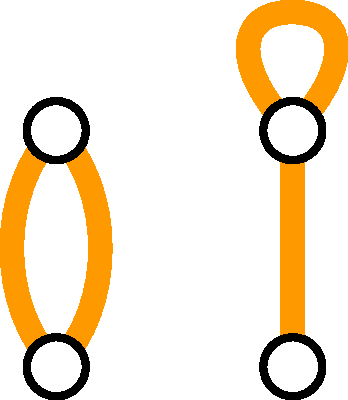
\includegraphics[width=.15\textwidth]{figures/graphexamples2.pdf}
  \caption{An edge bijection preserving incidence may not be an isomorphism for multigraphs.
  A self-loop might swap with a multiedge if the multiedge is not incident to additional edges.}
  \label{fig:looptomultiedge}
\end{figure}
This is the case for some automorphisms  of $\mathcal C S_{1,2}$ acting on region adjacency graphs.
Luo describes how a quotienting of  $S_{1,2}$ by a hyperelliptic involution gives
an isomorphism $\aaut \mathcal C S_{1,2} \to \aaut \mathcal C S_{0,5}$ \cite{MR1722024}.
An automorphism of $\mathcal C S_{1,2}$ bijects edges and preserves incidence of the region adjacency graph, but may not induce an isomorphism. The corresponding automorphism of $\mathcal C S_{0,5}$ induces an
isomorphism of the region adjacency graph, as in Figure \ref{fig:s12ands03}.




\begin{figure}[h!]
  \centering
  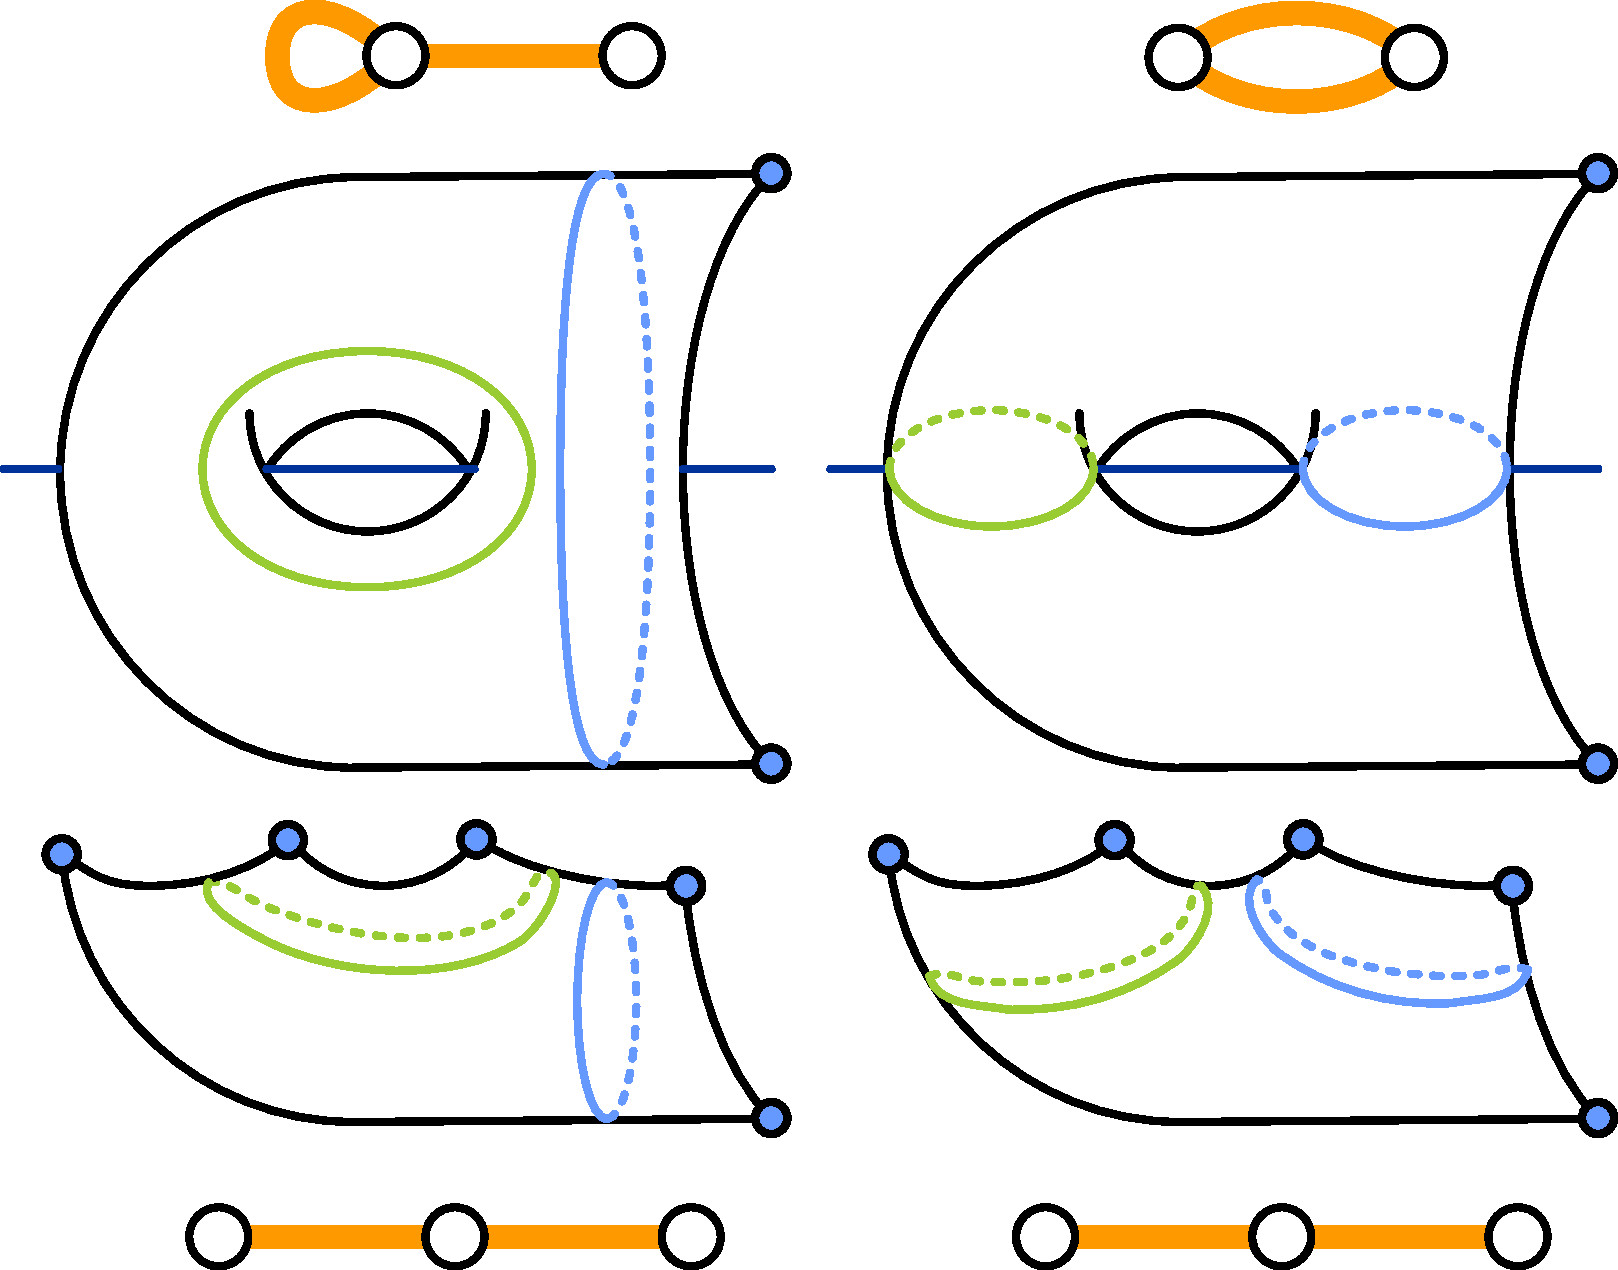
\includegraphics[width=.7\textwidth]{figures/s12ands03.pdf}
  \caption{(Top) Two nonisomorphic region adjacency graphs can be exchanged by an automorphism of $\mathcal C_{1,2}$,
  though the edge incidence relation is preserved.
  (Bottom)
  Such an automorphism of $\mathcal C S_{1,2}$ corresponds via hyperelliptic involution to a homeomorphism of $S_{0,5}$.}
  % An automorphism of $\mathcal C S_{1,2}$ bijects edges and preserves incidence of the region adjacency graph, but may not induce an isomorphism. The corresponding automorphism of $\mathcal C S_{0,5}$ induces an isomorphism of the region adjacency graph.}
  \label{fig:s12ands03}
\end{figure}

\end{example}



\begin{corollary}
  Curve complex automorphisms induce isomorphisms of
  region adjacency graphs of maximal simplices.

  Suppose that $3g+p\geq 5$  and $(g,p)\neq(1,2)$.
  Let $\phi \in \aaut \mathcal C S_{g,p}$
  and let $\Delta$ be a maximal simplex of $\mathcal C S_{g,p}$.
  Then $\mathcal G_\Delta$ and
  $\mathcal G_{\phi(\Delta)}$
  are isomorphic graphs.
  \label{cor:adjgraph}
\end{corollary}

\begin{proof}
  Any maximum simplex $\Delta$
  gives a pants decomposition of the surface $S_{g,p}$
  with $3g+p-3$ curves and $2g+p-2$ pairs of pants.
  So $\mathcal G^{simp}_\Delta$
  and
  $\mathcal G^{simp}_{\phi(\Delta)}$
  are simple, connected graphs with the same number of
  vertices and the same edge-incidence relations.
  Then by Whitney's Theorem \ref{thm:whitney},
  $\mathcal G^{simp}_\Delta$ is isomorphic to
  $\mathcal G^{simp}_{\phi(\Delta)}$.

  To see that self-loops are preserved, observe
  that as $\Delta$ cuts $S_{g,p}$ into pairs of pants,
  every vertex of $\mathcal G_\Delta$ has degree at most 3.
  Then if $e_c$ is a self-loop at vertex $v_R$,
  it is incident to exactly one other edge $e_x$
  that cannot be a self-loop, so $e_x$ is uniquely represented in $\mathcal G^{simp}_\Delta$.
  If $(g,p) \neq (1,2)$, then $e_x$ is incident to another edge $e_y$.
  Then $e_\phi(x)$ is
  also uniquely represented in the isomorphic graph $\mathcal G^{simp}_\Delta$
  and has a degree 1 vertex.
  Then in $\mathcal G^{simp}_\Delta$, $e_\phi(x)$
  is incident to $e_\phi(y)$, and $e_\phi(c)$ is incident to $e_\phi(x)$,
  but not $e_\phi(y)$ or any other edge, so $e_\phi(c)$   must be a loop at the vertex
  that is degree 1 in $\mathcal G^{simp}_{\phi(\Delta)}$.
\end{proof}


\begin{lemma}
  Automorphisms of the curve complex preserve the sides and topological type of curves.

  Suppose that $3g+p \geq 5$ and $(g,p)\neq(1,2)$.
  Let $\phi \in \aaut \mathcal C S_{g,p}$ and let $x$ be a curve.
  Then there is a homeomorphism of $S_{g,p}$ exchanging $x$ and $\phi(x)$.
  Furthermore, if $x$ is separating and $y,y'$ lie on the same side of $x$,
  then $\phi(y),\phi(y')$ lie on the same side of $\phi(x)$.
  \label{lemma:curvetype}
\end{lemma}
\begin{proof}
  We will characterize each topological type of curve
  by a combinatorial property of a corresponding region adjacency graph,
  and apply Lemmas
  \ref{lemma:adjgraph} and \ref{cor:adjgraph}.

  \begin{enumerate}[$\cdot$]
    \item Nonseparating curves:
    Observe that a curve $c$ is nonseparating if and only if
    there is a maximal simplex $\Delta$ such that $e_c$
    is a self-loop in the region adjacency graph $\mathcal G_\Delta$.
    \item Separating curves:
    Observe that if curve $x$ separates $S_{g,p}$
    $$
    S_{g,p} = S_{g',p'} \sqcup_c S_{g-g',p-p'+2}
    $$
    then the corresponding edge $e_x$ of the
    region adjacency graph
    $\mathcal G_\Delta$
    is a cut edge.
    More specifically, if
    $$\Delta = \Delta_+ \cup \{x\} \cup \Delta_-$$
    with $\Delta_+$ and $\Delta_-$
    the curves on each side of the separating curve $c$,
    then $e_x$ separates $\mathcal G_\Delta$
    $$\mathcal G_\Delta  - \{e_x\}  = \mathcal G_{\Delta_+} \sqcup  \mathcal G_{\Delta_-}$$
    into the components
    $\mathcal G_{\Delta_+}$, with
    $3g'+p'-3$ edges and genus $g'$,
    and $\mathcal G_{\Delta_-}$ with $3(g-g')+p-p'-1$ edges and genus $g-g'$.
  \end{enumerate}
  \end{proof}




\begin{remark}
For the closed surface $S_g$ the inclusion $S_{g}-\{q\} \hookrightarrow S_{g}$
induces a well defined puncture-forgetting projection map
$$
\rho_q: \mathcal C S_{g,1} \to \mathcal C S_g.
$$
by sending curves to their image.
Since we do not allow peripheral curves in $\mathcal C S_{g,1}$, no curve becomes nullhomotopic.
However, in the case of multiple punctures $P$,
the surface $S_{g,p}$ has curves bounding twice-punctured disks,
that may become peripheral if a puncture is forgotten.
Excluding these curves
gives a subcomplex $\mathcal C(S_{g,p},q) \subset \mathcal C S_{g,p}$
where the puncture-forgetting map is well-defined for puncture $q$.
$$
\rho_q: \mathcal C(S_{g,p},q) \to \mathcal C S_{g,p-1}
$$

Kent, Leininger, and Schleimer \cite{MR2599078}
show that this forgetful projection has
fibers described by Bass-Serre trees of the surface fundamental group
so that there is a fibration of the form
$$
\mathcal T \to \mathcal C(S_{g,p},q) \to \mathcal C S_{g,p-1}.
$$
More rigorously,
\end{remark}

\begin{theorem}
  Let $\Delta \subset \mathcal C S_{g,p}$
  be a simplex with interior point $x \in \Delta$.
  Then the fiber $\rho^{-1}_q(x)$ is
  $\pi_1 \left ( S_{g,p}, q \right )$-equivariantly
  homeomorphic to the tree $\mathcal T_\Delta$,
  the Bass-Serre tree for the splitting of
  $\pi_1 \left ( S_{g,p}, q \right )$
  determined by the multicurve $\Delta$.
  \label{thm:kent}
\end{theorem}

\begin{remark}
Observe that $\mathcal C(S_{g,p},q)$
is not characteristic in $C S_{g,p}$,
since in general automorphisms of $C S_{g,p}$ will permute the punctures.
Let $\aaut (\mathcal C S_{g,p},q) < \aaut \mathcal C S_{g,p}$
be the subgroup of $\aaut \mathcal C S_{g,p}$
that preserves the fibration
$\mathcal C(S_{g,p},q) \to \mathcal C S_{g,p-1}$, that is
$$\phi \left ( \rho_q^{-1}\rho_q(x) \right ) = \rho_q^{-1}\rho_q(\phi(x))$$
for every $x \in C(S_{g,p},q)$.

If $\phi \in \aaut \mathcal C(S_{g,p},q)$ then there is a well defined push-forward
automorphism of the less-punctured quotient $\mathcal CS_{g,p-1}$.
Define $\rho^\ast_q \phi \in \aaut \mathcal CS_{g,p-1}$
by
$$\left (  \rho^\ast_q \phi \right ) (x) = \rho_q \left(\phi (y) \right )$$
for any choice of $y \in \rho^{-1}_q(x)$. This is well defined since if $y' \in \rho^{-1}_q(x) =\rho^{-1}_q\rho_q(y)$
then
$$\phi(y') \in \phi(\rho^{-1}_q \rho_q y ) = \rho^{-1}_q \rho_q\phi( y )$$
by definition of $\aaut \mathcal C(S_{g,p},q)$.
Then this gives a pushforward map
$$
\rho_q^\ast : \aaut \mathcal (CS_{g,p},q) \to  \aaut \mathcal CS_{g,p-1}
$$
given by $\phi \mapsto \rho_q^\ast \phi$ as above.
\end{remark}

These automorphisms display the structure of the Birman exact sequence.

\begin{lemma}
  This diagram commutes
  $$
  \begin{tikzcd}
  1 \arrow[r]&
  \pi_1(S_{g,p-1},q) \arrow[r] \arrow[d]&
  \mcg^{\pm}(S_{g,p},q)  \arrow{r}{f_q} \arrow[d]&
  \mcg^{\pm}S_{g,p-1} \arrow[r] \arrow[d]&
  1 \\
  1 \arrow[r]&
  \pi_1(S_{g,p-1},q) \arrow{r}{\alpha}&
  \aaut \mathcal C (S_{g,p},q)  \arrow{r}{\rho^\ast_{q}}&
  \aaut \mathcal C S_{g,p-1} \arrow{r}&
  1 \\
  \end{tikzcd}
  $$
  and has exact rows when $\rho_{q}$ is surjective.
  \label{lemma:exact}
\end{lemma}



\begin{proof}
  The pushforward $\rho^\ast_q: \aaut \mathcal C (S_{g,p},q)  \to
  \aaut \mathcal C S_{g,p-1}$
  is defined by
  $$
  (\rho^\ast_q \phi) (x) = \rho_q( \phi(y))
  $$
  where $y \in \rho^{-1}_q(x)$. This is well defined since if $z \in \rho^{-1}_q(x)$
  then $\phi(z))  \in \rho^{-1}_q \rho_q (\phi(y))$ by definition of $\aaut \mathcal C (S_{g,p},q)$.


  The map $\alpha$ is defined by the first square,
  so it certainly commutes.
  And $\alpha$
  gives a well defined injection,
  since for any nontrivial loop $\gamma$
  there is a nonseparating curve $c$
  that intersects $\gamma$ so that the point pushing map
  $\alpha(\gamma)$ moves $c$, and $c \in \mathcal C (S_{g,p},q)$.

  The second square must commute,
  since if $[\psi] \in \mcg^\pm (S_{g,p},q)$
  is a mapping class and $c$ a curve of $S_{g,p}$,
  the homotopy class of $\psi(c)$ is the same if we first
  allow homotopies of the homeomorphism $\psi$ which do not fix $q$, or if we first consider the homeomorphism $\psi$
  up to homotopy fixing $q$, then homotope the curve $\psi(c)$ forgetting $q$.

  As in  Theorem \ref{thm:kent},
  the fiber $\rho^{-1}_q(x)$ of the projection
  $\rho_q: \mathcal  C (S_{g,p},q) \to \mathcal C S_{g,p}$
  for a curve $x$
  is homeomorphic to the Bass-Serre
  tree $\mathcal T_x$ given by the splitting $x$ specifies on $\pi_1(S_{g,p},q)$.
  Then the kernel $\ker \rho_{q}$ is a
  group acting faithfully on the tree $\mathcal T_\Delta$,
  so by the
  Fundamental Theorem of Bass–Serre Theory
  \ref{thm:bassserre},
  $\ker \rho^\ast_{q}$ is isomorphic to
  the fundamental group $\pi_1$ of the
  quotient graph of groups,
  but the corresponding graph of groups is
  exactly the Van Kampen splitting of $\pi_1$ induced by $x$.
  Thus
  $$\ker \rho^\ast_{q} = \mbox{image } \alpha \cong \pi_1(S_{g,p},q)$$
  and the second row is exact.
\end{proof}

We will show that, though curve complex automorphisms might not
preserve the fibers of $\rho_q$ for any particular puncture $q$, they do permute the fibers
of the puncture-forgetting projections $(\rho_q)_{q \in P}$.
We do so by proving the unique colorability of an arc complex.
Korkmaz's proof of Theorem \ref{thm:curvecomplex}
utilizes a slightly more general arc complex
allowing peripheral arcs \cite{MR1696431} and simplices of arcs that share endpoints.

\begin{definition}
  Define the pointed arc complex
  $\mathcal A S_{g,p}$
  to be the complex of homotopy classes of embedded
  non-peripheral arcs in $S_{g,p}$ with endpoints in $P$,
  where an arc is peripheral if
  it is a separating loop based at a single puncture
  and one of its sides is a punctured monogon of $S_{g,p}$.
  Two arcs or disks are adjacent in
  $\mathcal A S_{g,p}$ if their homotopy classes
  have disjoint representatives and share no punctures as endpoints.
  \label{def:ptarc}
\end{definition}

\begin{remark}
  The pointed arc complex $\mathcal A S_{g,p}$ has as vertices
  both arcs with two distinct
  endpoints and loops based at a single puncture.
  Since loops that are disjoint are always
  based at distinct punctures,
  there is an obvious way to color (in the graph-theoretic sense)
  the vertices of
  $\mathcal A S_{g,p}$ that are loops:
  assign a color to each puncture and all the loops based at that puncture.
  The arcs with distinct endpoints
  require two colors, however.
  We make a slight generalization of
  $k$-colorings to allow a privileged set of vertices that
  that require two colors.

  Recall from Definition \ref{def:color}
  that a $k,\eta$-coloring
  assigns to each vertex $x$ a set of $\eta(x)$ colors from $k$ options
  so that adjacent vertices have disjoint color sets.
\end{remark}


%#___________________
\begin{remark}
Margalit in \cite{MR2040283} discusses the
trinion pants complex.
Pants decompositions of $S_{g,p}$ are maximal simplices of
$\mathcal C S_{g,p}$,
with two such pants decompositions giving sharing
an edge in the pants complex if they differ
by a single pair of minimally intersecting curves.
Hatcher and Thurston
demonstrated the
pants complex (which they call \emph{markings}) of a surface
is connected and simply connected
in \cite{MR579573}.
We recall their result as the following lemma.
\end{remark}

\begin{lemma}
  \label{lem:maxsimppath}
  Let $\Delta,\Delta'$ be maximal $k$-simplicies of $\mathcal C S_{g,p}$.
  Then there is a sequence $\Delta = \Delta_0, \Delta_1, \ldots, \Delta_n=\Delta'$
  of maximal simplices such that
  $\Delta_i \cap \Delta_{i+1}$ is a $k-1$ simplex
  and the curves $c_i \in \Delta_i - \Delta_{i+1}$
  and $c'_i \in \Delta_{i+1} - \Delta_i$
  are contained in a single component $R$ of
  $S_{g,p} - \bigcup_{x \in \Delta_i \cap \Delta_{i+1}} x$.
  Further,
  $c_i,c'_i$ can be chosen to intersect once if $R \cong S_{1,1}$
  and twice if $R \cong S_{0,4}$.
  \label{lemma:pantspath}
\end{lemma}

\begin{remark}
Lemma \ref{lemma:pantspath}
in particular implies that for any two maximal $k$-simplicies
$\Delta,\Delta'$ contained in a $k$-colorable subgraph of $\mathcal C S_{g,p}$
the simplex $\Delta$ forces a coloring on $\Delta'$.
Bestvina, Bromberg, and Fujiwara note bounds on the chromatic number of the curve graph $\mathcal C S_{g,p}$
in \cite{MR3415065}.
Gaster, Greene, and Vlamis further develop the theory of  in \cite{2016arXiv160801589G}, where they additionally consider colorings of
a related arc complex that contains $\mathcal A S_{g,p}$ as a proper subcomplex, albeit with many more edge relations
\end{remark}

We will show that $\mathcal A S_{g,p}$ is uniquely colorable.

%#___________________

\begin{definition}
  \label{def:nest}
Fix an ordering $\sigma:P \to \{1,\ldots,p\}$ of the punctures
and let $x$ be a curve of $S_g$.
A $\sigma$-\emph{nest} of curves parallel to $x$
is the homotopy class in $S_{g,p}$
of an embedding
$$N: S^1 \times I \hookrightarrow S_{g,p}$$
such that $N$ is a homotopic to $x$ in $S_g$ by homotopy forgetting the punctures,
and image of $S^1 \times \{{\sigma(i)-1}/{(p-1)}\}$ is a loop based at puncture $\sigma^{-1}(i)$
that we refer to as the rib $N_i$.
The nest also gives a collection of $p-1$ arcs.
The  $i^{\mbox{th}}$ \emph{vertebra} of $N$ is the arc from $\sigma^{-1}(i)$ to $\sigma^{-1}(i+1)$ and given by
$$
N \left ( \{s_0\}\times  \left [ \frac{\sigma(i)-1}{p-1}, \frac{\sigma(i+1)-1}{p-1} \right]  \right )
$$
for the basepoint $s_0 \in S^1$.
We refer to $N(s_0 \times I)$ as the \emph{spine} of $N$.
\end{definition}


\begin{figure}[h!]
  \centering
  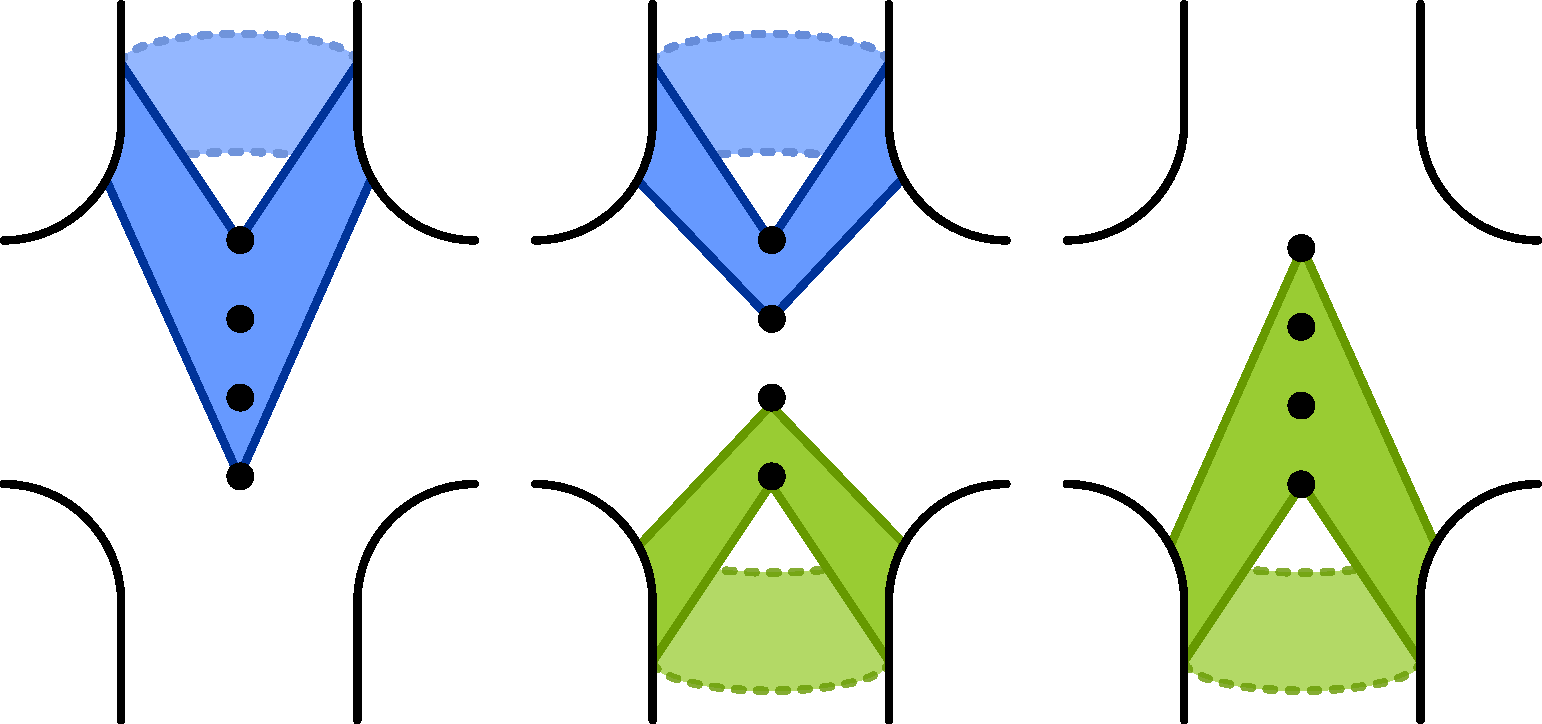
\includegraphics[width=.7\textwidth]{figures/corset.pdf}
  \caption{A color forcing path between nests parallel to disjoint curves.}
  \label{fig:corset}
\end{figure}


\begin{example}
  \label{example:nests}

  Observe that any nest $N$ in $S_{g,p}$
  specifies a maximal simplex  $\Delta_N$  in $\mathcal A S_{g,p}$.
  Further two $\sigma$-nests $N,N'$ respectively parallel to
  disjoint curves $x,x'$ of $S_{g,p}$
  specify a length $p$ sequence from $\Delta_N$ to $\Delta_{N'}$ of maximal simplices intersecting
  in codimension one faces as by replacing $N_i$ with $N'_i$, as in Figure \ref{fig:corset}.
  So $\Delta_{N}$ forces a $p$-coloring on $\Delta_{N'}$.

  \begin{figure}[h!]
    \centering
    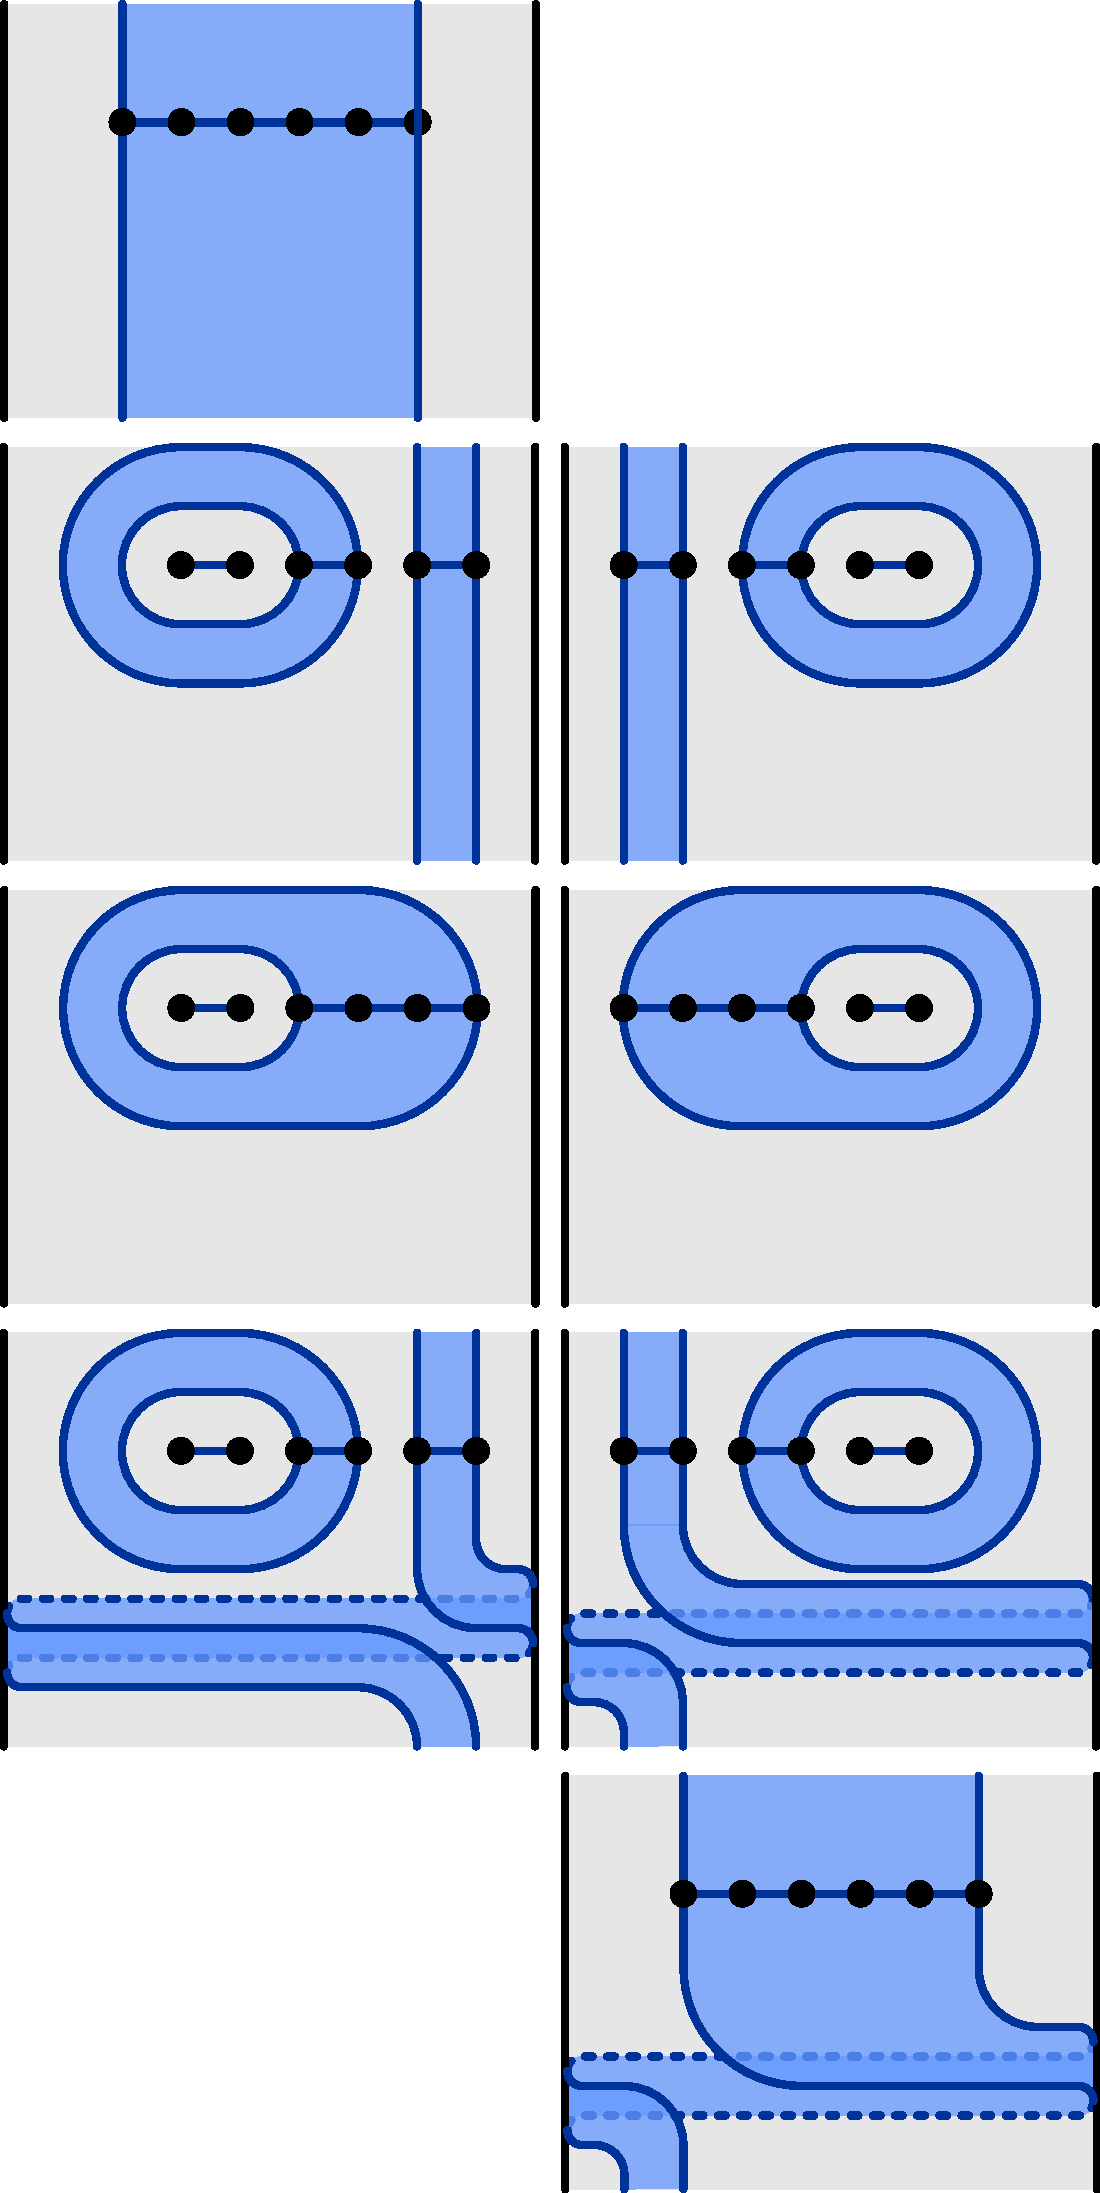
\includegraphics[width=.5\textwidth]{figures/nests.pdf}
    \caption{Two paths of simplices forcing  a coloring between nests parallel to intersecting curves.
    ``Pack'' curves on one boundary component of the nest into curves surrounding punctured disks,
    then unpack them parallel to a different curve of the unpunctured surface.
    Repeat this with the other boundary component of the nest.
    }
    \label{fig:nests}
  \end{figure}

  In fact even if $x$ and $y$ intersect $\Delta_{N}$ forces a $p$-coloring on $\Delta_{N'}$ if there are enough punctures.
  Consider two paths of maximal simplices intersecting
  in codimension one faces shown in Figure \ref{fig:nests}.
  First replace $N_1,N_2$ with the first vertebra $\alpha_{1,2} =N( {s_0}\times[\sigma(1)/(p-1), \sigma(2)/(p-1)])$
  between the punctures $\sigma(1)$ and $\sigma(2)$.
  Then iteratively we replace $N_i$ with the loop $\alpha_i$ based at $\sigma(i)$ and parallel to the
  boundary of a regular neighborhood of $\alpha_{i-1}$ for $i=3$ to $i=p$.
  Then replace $\alpha_i$ with $N'_i$ for $i=p$ to $i=3$ to obtain a simplex $\{\alpha_2, N'_3,\ldots, N'_p\}$.
  Starting from the other end of the spine we construct a similar path with the puncture order reversed to obtain a simplex $\{N'_1, \ldots, N'_{p}, \alpha_{p-1,p}\}$.
  Since $\{\alpha_2, N'_3,\ldots, N'_p\}$ and $\{N'_1, \ldots, N'_{p}, \alpha_{p-1,p}\}$
  together contain $\Delta_{N'}$,
  it must be that $\Delta_{N}$ forces a $p$-coloring on $\Delta_{N'}$.

  We will use this technique to demonstrate that $\Delta_N$ forces a coloring on all of $\mathcal A S_{g,p}$.
\end{example}






\begin{lemma}
  The pointed arc complex is uniquely colored by the punctures.

  Let $3g+p\geq6$.
  The pointed arc complex $\mathcal A S_{g,p}$
  admits a
  unique
  $p,\eta$-coloring,
  up to permutation of the colors,
  where $\eta(x)$ is the number of endpoints of the arc $x$.
  \label{lemma:paint}
\end{lemma}

\begin{proof}
  We will argue with a modification of the Putman trick \ref{putmancolor}.
  Observe that (since we exclude peripheral arcs)
  every maximal simplex of $\mathcal A S_{g,p}$
  has an arc with an end at every puncture.
  Observe that if $p \leq 2$ the result is trivial,
  so we assume $p \geq 3$.
  Let $f$ be any $p$-coloring of the
  arc complex $\mathcal A S_{g,p}$.

  \begin{figure}
    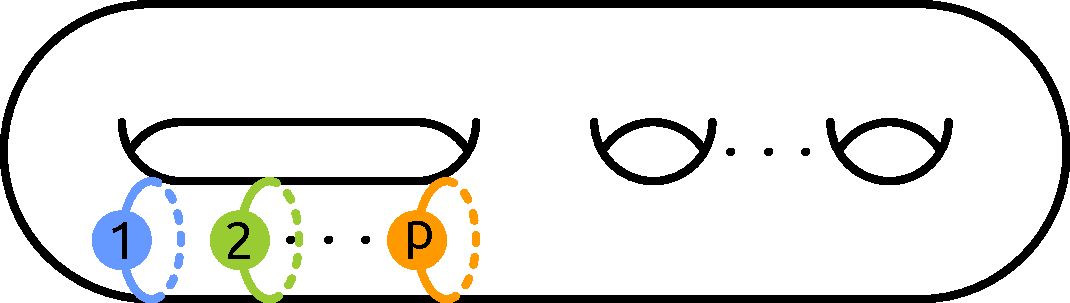
\includegraphics[width=.6\textwidth]{figures/pcolorgenus.pdf}
    \caption{A base collection of parallel nonseparating loops, as in a nest.}
    \label{fig:pcolorg}
  \end{figure}

  We first fix a collection $X$ of curves.
  If $g\geq1$, then $S_{g,p}$ has a nonseparating curve,
  and we let $X$ contain $p$ parallel nonseparating loops based at the punctures
  as in Figure \ref{fig:pcolorg}.


  If $g=0$ we take as $X=\{x_i\}_{i=1}^p$ to be as in Figure \ref{fig:pcolors}
  with $p-4$ parallel loops based at $p_2,\ldots,p_{p-2}$
  and 4 additional curves $x_1,x_2,x_{p-1},x_p$
  so that $x_1$, $x_2$ and $x_3$ pairwise intersect twice
  and are disjoint from all other curves of $X$,
  and similarly $x_p,x_{p-1},x_{p-2}$ pairwise intersect twice
  and are disjoint from all other curves of $X$.
  We will argue that each loop of $X$ must be colored differently.
  Observe that there is an arc
  $\alpha_{12}$
  from $p_1$ to $p_2$
  that is disjoint from all loops of $X$ except $x_1$ and $x_2$.
  Similarly
  there is  $\alpha_{p-1,p}$
  disjoint from all loops of $X$ except $x_p$ and $x_{p-1}$.
  So the collection $\alpha_{12},x_3,\ldots,x_{p-2},\alpha_{p-1,p}$
  require all $p$-colors to paint,
  and it must be that $f(x_1)\cup f(x_2) = f(\alpha_{12})$
  and $f(x_{p-1})\cup f(x_p) = f(\alpha_{p,p-1})$.
  So $X$ requires $p$-colors to paint.

  \begin{figure}
    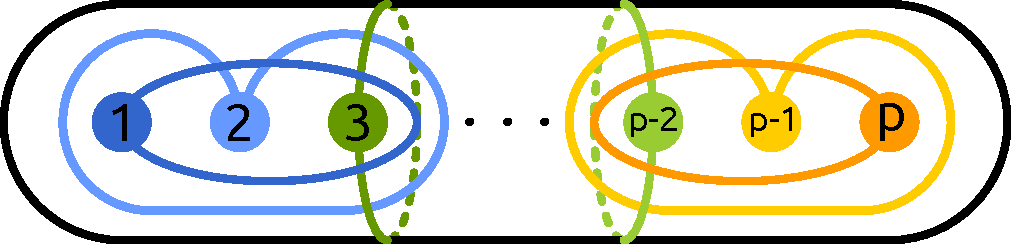
\includegraphics[width=.6\textwidth]{figures/pcolorspher.pdf}
    \caption{A base collection of mostly parallel loops in the punctured sphere.}
    \label{fig:pcolors}
  \end{figure}


  We may then assume, possibly after relabeling the colors,
  that $f$ colors the arcs of $X$ by their punctures.
  Applying Lemma \ref{putmancolor},
  we will show that the coloring on $X$ forces
  the coloring on all of $\mathcal A S_{g,p}$.
  Our technique will be to contruct paths with the group action
  of $\mcg S_{g,p}$ on $\mathcal A S_{g,p}$
  and show that $f$ is determined along these paths.
  Let $\alpha_{i,i+1}$ be an arc that is disjoint from
  all loops of $X$ except $x_i$ and $x_{i+1}$
  and contained in the annulus they bound if they are disjoint.
  Take as a generating set of $\mcg S_{g,p}$
  the Dehn half-twists along the arcs $\alpha_{i,i+1}$
  and the usual Humphrey's generators
  of Dehn twists about nonseparating curves
  that are disjoint from $X$, except for one curve $z$
  that intersects each loop of $X$ exactly once.

  We now claim that for $h \in H$ the
  coloring $f$ is determined on the loops $h\cdot X$
  by the coloring on $X$.
  We must consider several cases
  depending on whether $h$ is a twist or half-twist,
  and how $\alpha_{i,i+1}$ intersects $X$.
  These cases are considered in Figures \ref{fig:pcolor1}-\ref{fig:pcolor4}.
    \begin{figure}[h!]
      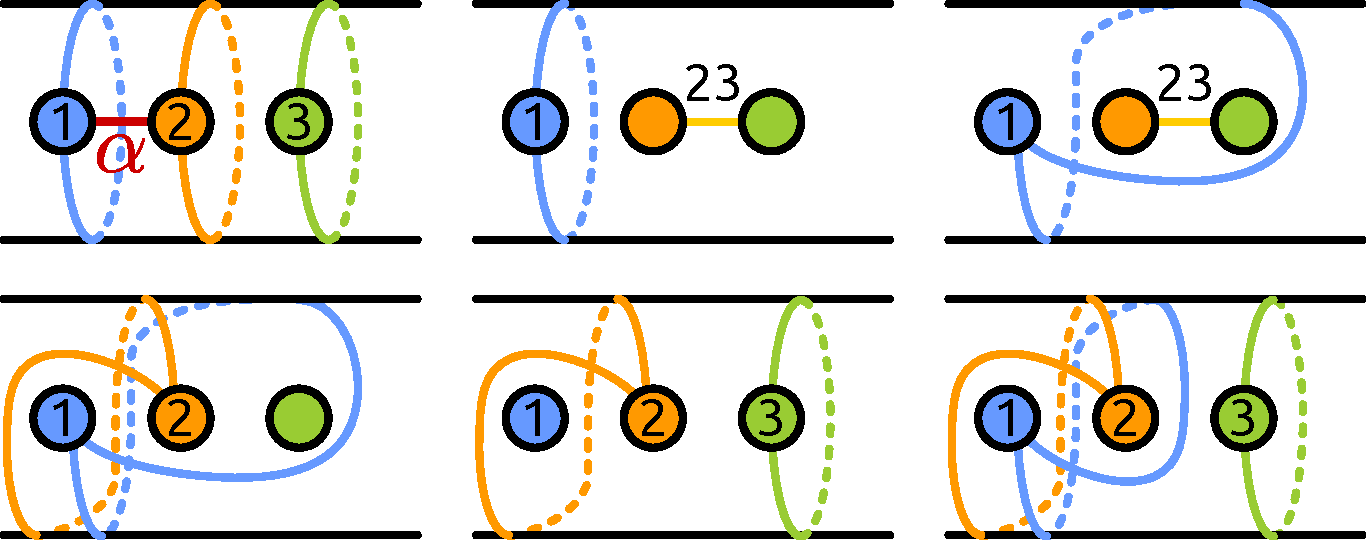
\includegraphics[width=.8\textwidth]{figures/pcolorsequence1.pdf}
      \caption{Case 1: The half-twist $h$ is about an arc $\alpha$
      in an annulus between $x_i$ and $x_{i+1}$ and disjoint from the other loops of $X$,
      as in the top left.
      The lower right shows $h(x_1)$, $h(x_2)$, and $h(x_3)=x_3$.
      Then if $f(x_i)=p_i$ the sequence of curve replacements shows
      that $f(h(x_i))=p_i$.
      }
      \label{fig:pcolor1}
    \end{figure}
    \begin{figure}[h!]
      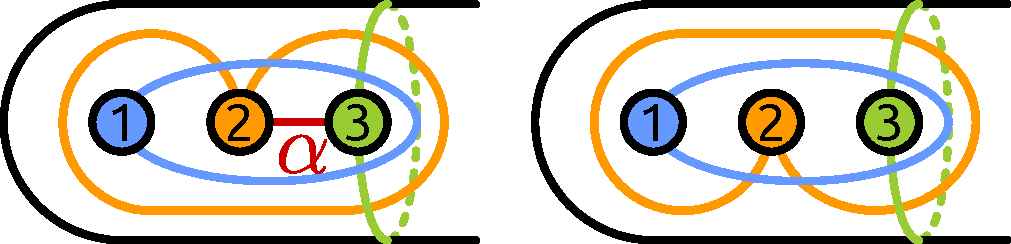
\includegraphics[width=.6\textwidth]{figures/pcolorsequence2.pdf}
      \caption{Case 2: The half-twist $h$ is about an arc $\alpha$
      $x_i$ and $x_{i+1}$ and disjoint from the other loops of $X$,
      where $x_i$ and $x_{i+1}$ intersect twice.
      We may assume the configuration on the left and note that
      $h(x_2)=x_3$, so that $f(h(x_3))$ must be $p_2$.}
      \label{fig:pcolor2}
    \end{figure}


    \begin{figure}[h!]
      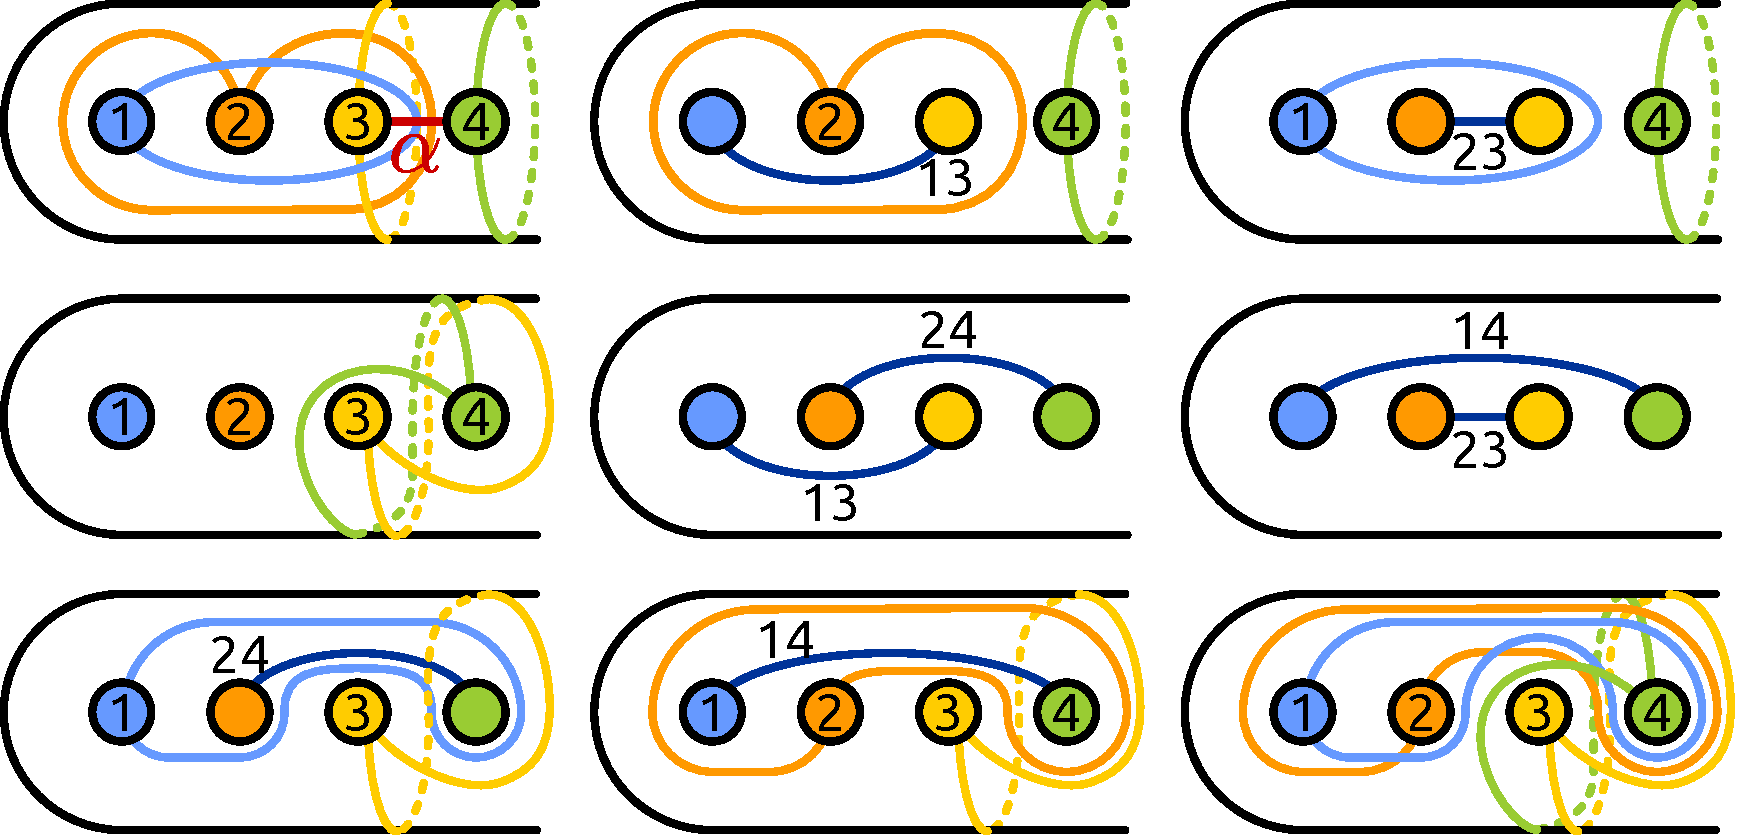
\includegraphics[width=\textwidth]{figures/pcolorsequence3.pdf}
      \caption{Case 3: The half-twist $h$ is about arc $\alpha$
      between disjoint curves $x_i$ and $x_{i+1}$,
      and $\alpha$ intersects other curves of $X$.
      We may assume the configuration on the top left.
      Then the image of $h$ is shown in the bottom right.
      Note that by Case 1, $f(h(x_3))=p_3$ and $f(h(x_4))=p_4$
      so that we need only determine $f(h(x_1))$ and $f(h(x_2))$.
      }
      \label{fig:pcolor3}
    \end{figure}
    \begin{figure}[h!]
      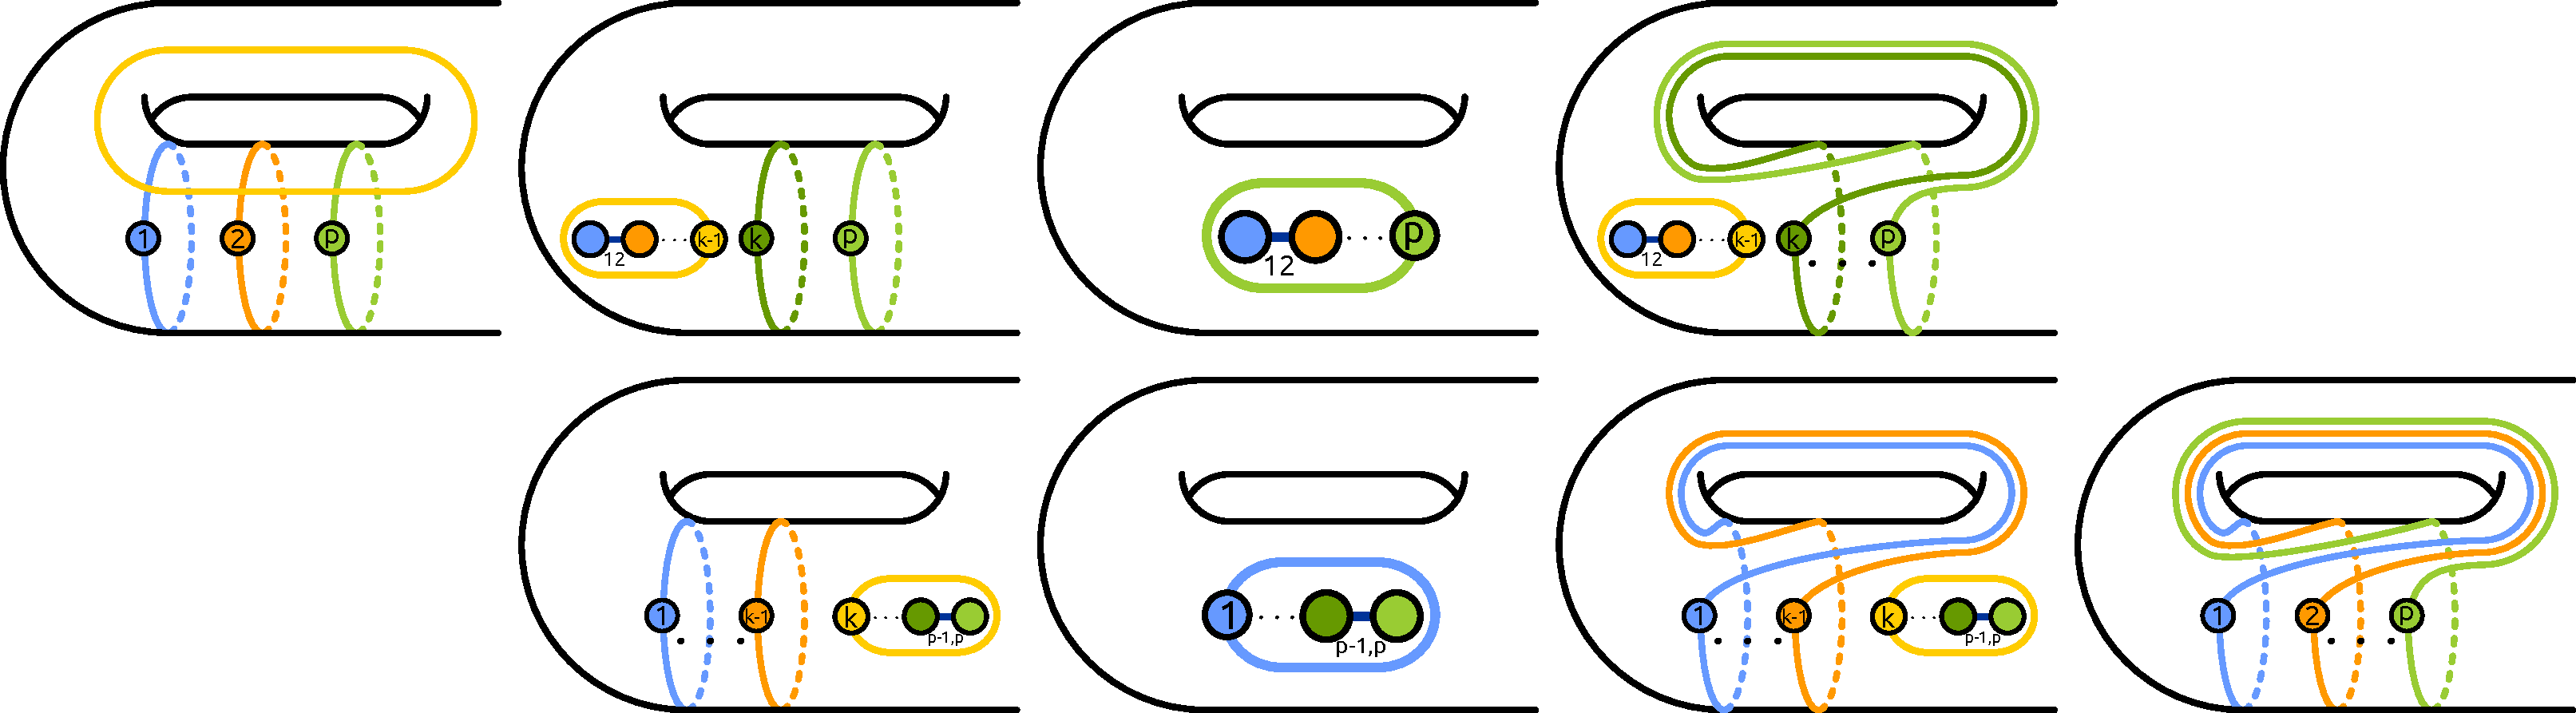
\includegraphics[width=1\textwidth]{figures/pcolorsequence4.pdf}
      \caption{Case 4: The Dehn twist $h=T_z$ about a nonseparating curve
      that links with the loops of $X$.
      We may assume the configuration of $X$ and $z$ as in the top left.
      The image $T_z(X)$ is shown in the bottom right.
      In the top row: Replace $x_1$ and $x_2$ with $\alpha_{1,2}$
      so that $f(\alpha_{12})=\{p_1,p_2\}$.
      Then iteratively replace $x_k$ with the loop $y_k$ separating
      $\alpha_{1,2},y_3, \ldots, y_{k-1}$ from the other punctures,
      so that $f(y_k)=p_k$ for $k=3,\ldots,p$.
      Then replace $y_k$ with $h(x_k)$ so that $f(T_z(x_k))=p_k$
      for $k=p, \ldots, 3$.
      A similar process reversing the order of the punctures
      as in the bottom row shows $f(T_z(x_k))=p_k$ for $k=1,\ldots,p-2$.
      }
      \label{fig:pcolor4}
    \end{figure}

  Observe that if $g \in \mcg S_{g,p}$
  we can write $g= h_n \cdots h_1$ with $h_i \in H$.
  And if the loops of $h_k \cdots h_1 \cdot X$ are painted by their punctures,
  then so are the loops of $h_{k+1} \cdots h_1 \cdot X$ by the above argument.

  Observe in the case of $g=0$ every curve is in $\mcg S_{g,p} \cdot X$.
  If $g \geq 1$ then $\mcg S_{g,p} \cdot X$ includes all nonseparating loops,
  and any separating loop $x$ is disjoint from $p-1$ mutually disjoint loops $x_1,\ldots, x_{p-1}$
  so that
  the color $f(x)$ is determined by
  the colors
  $f(x_i)$
  and so $f(x)$ must be colored by its puncture.
\end{proof}


\begin{lemma}
  Curve complex automorphisms induce
  arc complex automorphisms.

   There is a natural $\mcg^\pm S_{g,p}$ equivariant map
   $$\aaut \mathcal C S_{g,p} \to \aaut \mathcal A S_{g,p}.$$
  \label{lemma:annulus}
\end{lemma}

\begin{proof}
  By Lemma \ref{lemma:curvetype}
  automorphisms of $\mathcal S_{g,p}$
  preserve the class of two curves.
  Observe that curves $c,c'$ of $S_{g,p}$
  bound a punctured annulus if and only if there
  is a maximal simplex $\Delta \subset \mathcal C S_{g,p}$
  containing $c,c'$
  so that in the region adjacency graph $\mathcal G_\Delta$,
  the edges $e_c$ and $e_{c'}$ are incident
  at a degree 2 vertex $v_a$.
  Then applying Lemma \ref{cor:adjgraph}
  $\phi(c)$ and $\phi(c')$ must cobound a punctured annulus.

  Let $\phi \in \aaut \mathcal C S_{g,p}$
  and let $a$ be an punctured annulus $\mathcal A S_{g,p}$
  with bounding curves $c,c'$.
  If $(g,p) \neq (1,2)$ then $c,c'$ uniquely specify the annulus.
  Then $\phi(c),\phi(c')$ specify cobound a punctured annulus $\phi_\ast(a)$.

  Finally $a,a'$ are disjoint arcs if and only if
  there is a maximal simplex $\Delta \subset \mathcal C S_{g,p}$
  such that the bounding curves of regular neighborhoods of
  $a$ and $a'$
  are in $\Delta$.
  Then $a$ and $a'$ are represented by distinct
  vertices $v_a$ and $v_{a'}$ of $\mathcal G_\Delta$.
  So $a$ and $a'$ are disjoint if and only if
  $\phi_\ast (a)$ and $\phi_\ast (a')$ are disjoint.

  Thus $\phi_\ast : \mathcal A S_{g,p} \to \mathcal A S_{g,p}$
  is an isomorphism.
\end{proof}





\begin{lemma}
  Curve complex automorphism permute puncture-projection fibers.

  Let $\phi \in \aaut \mathcal C S_{g,p}$ for $3g+p \geq 6$.
  Then if $x,y$ are curves of $S_{g,p}$ with
  $\rho_q(x)=\rho_q(y)$,
  then there is a puncture $q' \in P$ such that
  $\rho_{q'}(\phi(x))=\rho_{q'}(\phi(y))$.
  \label{lemma:fibers}
\end{lemma}

\begin{proof}
  Consider the structure of $\rho^{-1}_q(\rho_q(x))$.
  We have it is a subtree of $\mathcal C S_{g,p}$
  with $x,x' \in \rho^{-1}_q(\rho_q(x))$
  adjacent if and only if they bound an annulus punctured by $q$.
  Then we have a path $x=x_0, \ldots, x_n =y$
  such that $x_i,x_{i+1}$ bound an annulus punctured by $q$.
  Using \ref{lemma:annulus}
  we have $\phi(x_i),\phi(x_{i+1})$ bound an annulus
  punctured by some $q_i$.
  Then since $x_i,x_{i+1},x_{i+2}$ bound
  annuli  punctured by $q$ that
    are the regular neighborhoods of
  loops $a_i,a_{i+1} \in \mathcal A S_{g,p}$ based at $q$.
  Then
  $\phi(x_i),\phi(x_{i+1}), \phi(x_{i+2})$
  bound annuli that are the regular neighborhoods
  of loops $\phi_\ast(a_i), \phi_\ast(a_{i+1})$.
  By Lemma \ref{lemma:paint}
  $\phi_\ast(a_i)$ and $\phi_\ast(a_{i+1})$
  are based at a common point $q'$.
\end{proof}


\begin{proof}[Proof of Theorem \ref{thm:addpunc}]
  Assume that the natural map
  $$
  \begin{tikzcd}
  \mcg^{\pm}S_{g,p-1} \arrow{r}{\gamma}& \aaut \mathcal C S_{g,p-1}
  \end{tikzcd}
  $$
  is an isomorphism.
  Then by Lemma
  \ref{lemma:exact}
  the following diagram commutes
  $$
  \begin{tikzcd}
  1 \arrow[r]&
  \pi_1(S_{g,p-1},q) \arrow[r] \arrow{d}{\alpha}&
  \mcg^{\pm}(S_{g,p},q)  \arrow{r}{f_q} \arrow{d}{\beta}&
  \mcg^{\pm}S_{g,p-1} \arrow[r] \arrow{d}{\gamma}&
  1 \\
  1 \arrow[r]&
  \pi_1(S_{g,p-1},q) \arrow{r}&
  \aaut \mathcal C (S_{g,p},q)  \arrow{r}{\rho_q}&
  \aaut \mathcal C S_{g,p-1} \arrow{r}&
  1. \\
  \end{tikzcd}
  $$
  and since $\gamma f_q = \rho_q \beta$ is a surjection we have
  that $\rho_q$ is a surjection and the rows are exact.
  By the Five Lemma $\beta$ is an isomorphism.

  Let $\phi \in \aaut \mathcal C S_{g,p}$.
  We have that by Lemma
  \ref{lemma:fibers} that
  $\phi$ permutes the fibers $\{\rho^{-1}_q\}$,
  so there is $\psi \in \mcg^{\pm}S_{g,p}$
  so that $\psi \in \aaut \mathcal C S_{g,p}$
  is such that $\psi \phi$ maintains the fibers
  $\rho^{-1}_q$.
  So $\psi \phi \in \aaut \mathcal C(S_{g,p},q)$.
  But then there is $\psi' \in \mcg^{\pm}S_{g,p}$
  so that $\psi \phi = \psi'$.
  But then $\phi = \left ( \psi^{-1}\psi' \right)$
  is also induced by a mapping class we have the natural map
  $$
  \begin{tikzcd}
  \mcg^{\pm}S_{g,p} \arrow{r} & \aaut \mathcal C S_{g,p}
  \end{tikzcd}
  $$
  is an isomorphism.
\end{proof}


\section{Spheres and Punctures}
\label{sect:spherepunc}

The main theorem of this section is the following


\outpunc*

The proof is directly analogous to our proof of Theorem
\ref{thm:addpunc}.
We will use a the structure of the puncture forgetful map and induct on the number of punctures.
A base, unpunctured case is considered by the Theorem of Aramayona and Souto \cite{souto}.

\aramsouto*

We will show that automorphisms of the punctured sphere complex
respect the fibration induced by forgetting punctures,
so that adding additional punctures expands the automorphism group
of the complex of spheres according to a Birman exact sequence.

\begin{theorem}
  If the natural map
  $$
  \oout_{n,p} \to  \aaut \mathcal  S_{n,p}
  $$
  is an isomorphism, then so is
  $$
  \oout_{n,p+1} \to  \aaut \mathcal  S_{n,p+1}
  $$
  \label{thm:outpunc}
\end{theorem}

\begin{definition}
  As in Definition \ref{def:graphadj} for surfaces, if
   $\Delta \subset \mathcal S_{g,p}$ is a simplex
  the \emph{region adjacency graph}
  $\mathcal G_\Delta$
  of $\Delta$
  is the graph whose vertices are the connected components
  of the cut manifold
  $$
  M_{n,p} - \bigcup_{x \in \Delta} x
  $$
  with an edge $e_x$ for every sphere $x$ and with
  the edge $e_x$ incident to the connected components it bounds.
  We will also consider the graph simplification
  $\mathcal G^{simp}_\Delta$.
\end{definition}

\begin{lemma}
  Sphere complex automorphisms preserve edge incidence of region adjacency graphs.

  Let $\phi \in \aaut \mathcal S_{n,p}$ and let $\Delta$ be a simplex of $\mathcal S_{n,p}$ with adjacency graph $\mathcal G_\Delta$.
  Then $e_x, e_{x'}$ are incident edges of $\mathcal G_\Delta$
  if and only if $e_{\phi(x)}, e_{\phi(x')}$ are incident
  edges of $\mathcal G_\phi(\Delta)$.
  \label{lemma:outlinegraph}
\end{lemma}

\begin{proof}
  We will argue that the induced bijection  $\phi_\ast$
  between the edges of $\mathcal G_\Delta$ and the edges of $\mathcal G_{\phi(\Delta)}$ preserves incidence.

  Let $x,x' \in \Delta$ be distinct spheres of $M_{n,p}$.
  Suppose that the associated edges $e_x$ and $e_x'$
  of $\mathcal G_\Delta$.
  It suffices to show that $e_x$ and $e_{x'}$ are incident if and only if there is a third $y \in \Delta$ with $y$
  intersecting $x$ and $x'$ but no other sphere of $\Delta$.
  In that case $e_{\phi(x)}$ and $e_{\phi(x')}$ are incident if and only if there is no third $\phi(y) \in \phi(\Delta)$ with $\phi(y)$
  intersecting $\phi(x)$ and $\phi(x')$ but no other sphere of $\phi(\Delta)$.
  So $\phi$ induces an incidence-preserving edge bijection between $\mathcal G_\Delta$ and $\mathcal G_{\phi(\Delta)}$.

  Suppose that $e_x$ and $e_{x'}$ are incident.
  Then there is a region $R$ of $M_{n,p}-\bigcup_{z \neq x,x'}z$
  containing $x$ and $x'$, and since every region of
  $M_{n,p}-\bigcup_{z \in \Delta}z$ contains at least an $M_{0,3}$,
  it must be that $R$ contains an $M_{1,2}$ or $M_{0,5}$.

  If $R$ contains an $M_{1,2}$ the subcomplex of spheres in $R$ contains a copy of $\mathcal S_{1,2}$ and so must have infinite diameter. So there must be a sphere $y$ in $R$ that intersects both $x$ and $x'$. Since $y$ is in $R$, it intersects no other sphere of $\Delta$.

  If $R$ is simply connected then it must have a copy of $M_{0,5}$
  and $x$ and $x'$ are essential and separating in $R$.
  Then there are two boundary spheres $y',y''$ of $R$ with a path $\alpha$ between them that passes through both $x$ and $x'$. Let $y$ be the boundary of a regular neighborhood of $\alpha \cup y' \cup y''$ in $R$. Then $y$ intersects both $x$ and $x'$, but since $y$ is in $R$, $y$ does not intersect any other sphere of $\Delta$.

  Suppose that $e_x$ and $e_{x'}$ are not incident.
  Then there is a collection of spheres $\Delta' \subset \Delta$
  that separate $x$ from $x'$ in $M_{n,p}$.
  So any sphere intersecting $x$ and $x'$ must also intersect a sphere of $\Delta$.
\end{proof}



\begin{corollary}
  Sphere complex automorphisms preserve the adjacency graphs of maximal simplices.

  Let $3n+p\geq 6$.
  Let $\phi \in \aaut \mathcal S_{n,p}$ and let $\Delta$ be a maximal simplex. Then $\mathcal G_\Delta$ and $\mathcal G_{\phi(\Delta)}$ are isomorphic.
  \label{lemma:outadjgraph}
\end{corollary}

\begin{proof}
  Any maximum simplex $\Delta$ contains
  $3n+p-3$ spheres and cuts $M_{n,p}$ $2n+p-2$ copies of  $M_{0,3}$.
  So $\mathcal G^{simp}_\Delta$ and $\mathcal G^{simp}_{\phi(\Delta)}$
  are simple, connected graphs with the same number of vertices and the same edge incidence relations.
  So by Whitney's Theorem  \ref{thm:whitney},
  $\mathcal G^{simp}_\Delta$ and $\mathcal G^{simp}_{\phi(\Delta)}$
  are isomorphic.

  To see that self-loops are preserved,
  observe that as $\Delta$ cuts $M_{n,p}$ into copies of $M_{0,3}$,
  every vertex of $\mathcal G_\Delta$ has degree at most 3.
  Then if $e_x$ is a self-loop at vertex $v_R$ it is incident to exactly one other edge $e_{x'}$ that cannot be a self-loop or have a parallel edge since $v_R$ is degree 3.
  So $e_{\phi(x')}$ has a degree one vertex in $\mathcal G^{simp}_{\phi(\Delta)}$.
  Since $3n+p-3\geq 3$ we have $\mathcal G_{\phi(\Delta)}$
  has at least 3 edges.
  So if both vertices of $e_{\phi(x')}$
  are degree one in $\mathcal G^{simp}_{\phi(Delta)}$, then $\mathcal G_{\phi(Delta)}$
  has two vertices with a self loop at each.
  So $e_{\phi(x)}$ is a self loop.
  If $e_{\phi(x')}$ has only one degree one vertex in $\mathcal G^{simp}_{\phi(Delta)}$, then $e_{\phi(x)}$ is only incident to $e_{\phi(x')}$. So $e_{\phi(x)}$ must be a self loop in  $\mathcal G_{\phi(\Delta)}$.

  If $\phi$ preserves both the graph simplification and the self loops of $\mathcal G_\Delta$, it must be that $\phi$ also preserves the multi-edges, and so $\phi$ induces a graph isomorphism.
\end{proof}

\begin{lemma}
  Sphere complex automorphisms preserve the topological type of spheres, and the sides of the spheres.

  Let $3n+p\geq 6$.
  Let $\phi \in \aaut \mathcal S_{n,p}$.
  Let $x$ be a sphere of $M_{n,p}$.
  Then $x$ and $\phi(x)$ have the same topological type.
  Further if $x$ is separating and $y,y'$ are spheres in the same connected component of $M_{n,p}-x$, then $\phi(x)$ is separating and $\phi(y),\phi(y')$ are
  in the same connected component of $M_{n,p}-\phi(x)$.
  \label{lemma:outspheretype}
\end{lemma}

\begin{proof}
    By Lemma \ref{lemma:outadjgraph}
    it suffices to characterise the topological type and sides of a sphere in terms of the region adjacency graph of a maximal simplex.
    \begin{enumerate}[$\cdot$]
    \item Nonseparating spheres:
    Observe that $x$ is a nonseparating sphere if and only if there is a maximal simplex $\Delta$ in that the corresponding edge $e_x$ is a self-loop in the region adjacency graph $\mathcal G_\Delta$.
    \item Separating spheres:
    Observe that if $x$ separates $M_{n,p}$
    $$
    M_{n,p} = M_{n',p'} \sqcup_x M_{n-n',p-p'+2}
    $$
    if and only if the corresponding edge $e_x$ of the region
    adjacency graph $\mathcal G_\Delta$ is a cut edge.
    More specifically, if
    $$
    \Delta=\Delta_+ \cup \{x\} \cup \Delta_-
    $$
     with $\Delta_+$ and $\Delta_-$ the spheres on each side of $x$,
     then $e_x$ separates $\mathcal G_\Delta$
     $$
     \mathcal G_\Delta - e_x = \mathcal G_{\Delta_+} \sqcup \mathcal G_{\Delta_-}
     $$
     into the components $\mathcal G_{\Delta_+}$
     with $3n'+p'-3$ edges and rank $n'$,
     and $\mathcal G_{\Delta_-}$ with
     with $3(n-n')+p-p'-1$ edges and rank $n-n'$.
  \end{enumerate}
\end{proof}

\begin{remark}
  Consider the inclusion that ignores the puncture $q$
  $$i_q: M_{n,p} \hookrightarrow M_{n,p-1}.$$
  Then for the homotopy class $[x]$ of a sphere
  in $M_{n,p}$ we have the class $[i_q(x)]$ in $M_{n,p-1}$
  by forgetting the puncture $q$.
  Separating spheres of $M_{n,p}$ bounding a copy of $S^3$ containing only $q$ and one other puncture
  will become non-essential in this inclusion,
  but other homotopy classes of spheres have well defined
  essential representatives up to homotopy forgetting $q$.

  Let $\mathcal S_{n,p}^{(q)} \subset \mathcal S_{n,p}$
  be the subcomplex for which the puncture forgetful map
  $\rho_q: [x] \mapsto [i_q(x)]$ is well defined.
  So we have a surjective projection map
  $$
  \rho_q: \mathcal S_{n,p}^{(q)} \to \mathcal S_{n,p-1}.
  $$

As in the case for surfaces, the fibers of this map are Bass-Serre trees.
% Let $\Delta$ be a simplex in $\mathcal S_{n,p-1}$.
% Let $\Delta'$ be a simplex of $\mathcal S_{n,p}$ such that $\rho_q(\Delta')=\Delta$.
Let $x$ be a sphere of $\mathcal S_{n,p-1}$.
Homotope $x$ in $M_{n,p-1}$ so that it is pointed at $q$.
Then the two boundary  spheres of a regular neighborhood of $x$ in $M_{n,p-1}$ gives a well edge of $\rho^{-1}_q(x) \subset \mathcal S_{n,p}$.
Let $\Gamma$ be the corresponding
be the graph of groups given by the splitting of $F_n=\pi_1(M_{n,p-1},q)$.
So the vertices of $\Gamma$ are the components of
$M_{n,p-1}-x$ with vertex groups given by the $\pi_1$ of the component,
and an edge with trivial edge group between two components if $x$ is separating, or a self-loop if $x$ is nonseparating.
Then there is a an isomorphism between
$\rho_q^{-1}(x)$ and the Bass-Serre tree $\tilde \Gamma$
given by associating every edge $xx'$ of $\rho_q^{-1}(x)$
with the edge of $\tilde \Gamma$ given by $uv$
if
$$
\mbox{stab}_{\pi_1(M_{n,p-1},q)}(u)
\ast
\mbox{stab}_{\pi_1(M_{n,p-1},q)}(v)
$$
is the splitting specified
by the pointed sphere at $q$ whose regular neighborhood in $M_{n,p}$ has boundary spheres
$x$ and $x'$.
\end{remark}

% \begin{lemma}
%   The fiber of the puncture forgetful map is isomorphic to the Basse Serre tree of the splitting
%   \label{lemma:outfibershape}
% \end{lemma}

\begin{definition}
  Let $\aaut(\mathcal S_{n,p},q) < \aaut \mathcal S_{n,p}$
  be the subgroup preserving the fibration of
  the forgetful map $\rho_p$.
  That is $\phi \in \aaut(\mathcal S_{n,p},q)$
  if
  $$
  \phi \left( \rho_p^{-1}\rho_p(x) \right)
  =
  \rho_p^{-1}\rho_p( \phi(x))
  $$
  for all spheres $x$.
\end{definition}

\begin{lemma}
  This diagram commutes
  $$
  \begin{tikzcd}
  1 \arrow[r]&
  \pi_1(M_{n,p-1},q) \arrow[r] \arrow[d]&
  \oout_{n,p}^{(q)}  \arrow{r}{f_q} \arrow[d]&
  \oout_{n,p-1} \arrow[r] \arrow[d]&
  1 \\
  1 \arrow[r]&
  \pi_1(M_{n,p-1},q) \arrow{r}{\alpha}&
  \aaut (\mathcal S_{n,p}, q)  \arrow{r}{\rho^\ast_{q}}&
  \aaut \mathcal S_{n,p-1} \arrow{r}&
  1 \\
  \end{tikzcd}
  $$
  and has exact rows when $\rho_{q}$ is surjective.
  \label{lemma:exactspheres}
\end{lemma}

\begin{proof}
  The map $\alpha$ is defined by the first square, so it commutes.
  The map $\alpha$ is injective, since
  for any loop $\gamma$ based at $q$,
  there is a nonseparating sphere $x$ intersecting $\gamma$
  so that the push map $\alpha(\gamma)$ acts non-trivially on $x$ and so cannot be the identity on $\mathcal S_{n,p}^{(q)}$.

  The second square must commute,
  since if $[\psi] \in \oout_{n,p}^{(q)}$
  is a mapping class of $M_{n,p}$ and $x$ a sphere of $M_{n,p}$,
  the homotopy class of $\psi(x)$ is the same if we first
  forget that the homeomorphism $\psi$ fixes $q$, or if we first allow $\psi$ with
  $q$ fixed then homotope the sphere $\psi(x)$ forgetting $q$.

  A fiber $\rho^{-1}_q(x)$ of the forgetful map
  $\rho^\ast_q: \mathcal  S_{n,p}^{(q)} \to \mathcal  S_{n,p-1}$
  is isomorphic to the Bass-Serre tree associated to the splitting.
  Then the kernel $\ker \rho^\ast_{q}$ is a
  group acting on the tree $\mathcal T_\Delta$,
  so by the
  Fundamental Theorem of Bass–Serre Theory
  \ref{thm:bassserre},
  $\ker \rho^\ast_{q}$ is isomorphic to
  the fundamental group $\pi_1$ of the
  quotient graph of groups,
  but the corresponding graph of groups is
  exactly the Van Kampen splitting of $\pi_1$ induced by $x$.
  Thus
  $$\ker \rho^\ast_{q} = \mbox{image } \alpha \cong \pi_1(S_{g,p},q)$$
  and the second row is exact.
\end{proof}

\begin{remark}
  The edges of the fibers of the forgetful map
  are between two spheres that cobound a
  $S^2 \times I$
  punctured by $q$.
  Such spheres are specified by the boundaries of regular neighborhoods of pointed spheres of $M_{n,p}$,
  so we consider the associated complex.
\end{remark}

\begin{definition}
  Let $\mathcal{PS}_{n,p}$
  be the \emph{pointed sphere complex} defined as follows.
  Let the vertices of $\mathcal{PS}_{n,p}$
  be either
  \begin{enumerate}[(1.)]
    \item pointed spheres in $M_{n,p}$, i.e. homotopy classes of maps
    $(S^2,s_0) \to (M_{n,p},P)$ where $s_0$ is a basepoint of the 2-sphere $S^2$ or else
    \item unpointed spheres that bound a twice punctured ball
  \end{enumerate}
  A collection of pointed spheres in $M_{n,p}$ span a simplex
  of $\mathcal{PS}_{n,p}$ if they have disjoint representatives, including the basepoints.
\end{definition}

\begin{definition}
As in Definintion  \ref{def:nest}, fix an order $\sigma: P \to \{1,\ldots, p\}$
let a $\sigma$-\emph{nest} of curves parallel to a sphere $x$
as the homotopy class in $M_{n,p}$
of an embedding
$$N: S^2 \times I \hookrightarrow S_{g,p}$$
such that $N$ is a homotopic to $x$ in $S_g$ by homotopy forgetting the punctures.
The image of $S^1 \times \{{\sigma(i)}/{(p-1)}\}$ is a pointed sphere based at puncture $\sigma(i)$
that we refer to as the pointed sphere $N_i$.
\end{definition}

\begin{lemma}
  The pointed sphere complex is uniquely colorable.

  % There is $p$-coloring of the 1-skeleton of $\mathcal S_{n,p}$ given by the puncture labels. Further, it is the unique $p$-coloring of
  % $\mathcal S_{n,p}$ up to permutations of the colors.
  Let $\eta(x)$ be 1 if $x$ is a pointed sphere and 2 if $x$ is an unpointed sphere that bounds a twice punctured ball of $M_{n,p}$.
  There is a unique $k,\eta$-coloring of $\mathcal {PS}_{n,p}$ given by the puncture labels.
  Further it is the only $k,\eta$-coloring up to relabeling of the $k$ colors.
  \label{lemma:outpaint}
\end{lemma}

\begin{proof}
  The argument is by the color modified Putman Lemma \ref{putmancolor}.
  Observe that if $p \leq 2$ or $n=0$ the result is trivial, so we assume $p \geq 3$ and $n \geq 1$.
  Let $f$ be any $p,\eta$-coloring of the pointed sphere complex $\mathcal{PS}_{n,p}$.

  Choose a maximal collection of nonseparating spheres $x_{a_1},\ldots,x_{a_n}$ of $M_{n,p}$
  and let $x_{b_1}, \ldots, x_{b_p}$.
  Let $H$ be the generating set of $\oout_{n,p}$ consisting of the transpositions
    $\sigma^a_{i} = (a_i a_{i+1})$
    and $\sigma^b_{i} = (b_i b_{i+1})$,
    the inversion $\iota_1$ at $a_1$ if $n=1$ or else the inversion $\iota_2$,
    the transvection $\tau_{12}$ with $a_1 \mapsto a_1a_2$ if $n\geq 2$,
    and the conjugation $\gamma_{11}$ with $b_1 \mapsto a_1b_1a_1^{-1}$.



  Let $V$ be the nest of $p$  nonseparating spheres all parallel to $x_{a_1}$
  so that $v_i$ is based at $x_{b_i}$  and separates $x^+_{a_1}, x_{b_1}, \ldots, x_{b_{i-1}}$ from
  the other spheres of $M_{n,p}$ cut along $x_{a_1},\ldots, x_{a_p}$, as in Figure \ref{fig:ptspherenest}.

  \begin{figure}[h!]
    \centering
    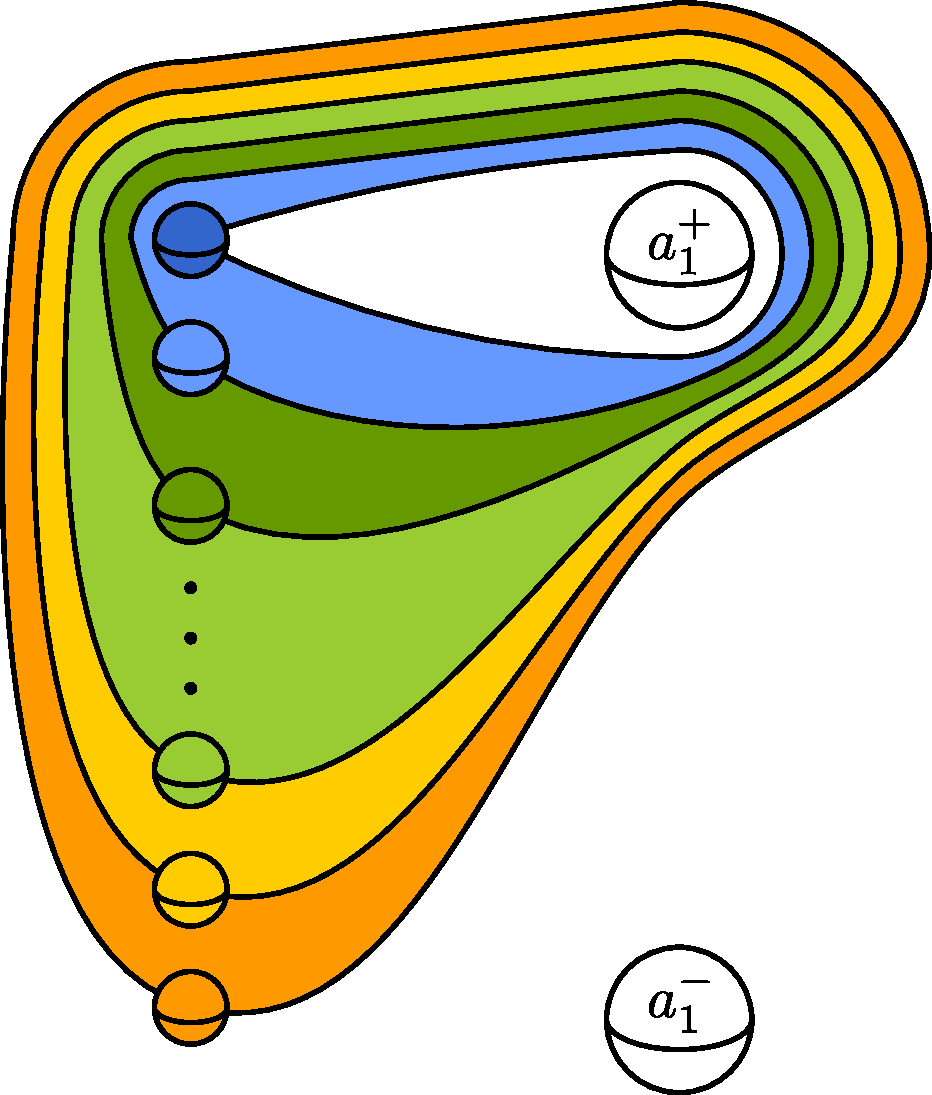
\includegraphics[width=.3\textwidth]{figures/ptspherenest.pdf}
    \caption{A nest of $p$ pointed spheres requires $p$ distinct colors.}
    \label{fig:ptspherenest}
  \end{figure}


  Since they are all disjoint they form a $p$-clique that requires they must be distinctly colored.
  We may assume, possibly after relabeling, that $f$ colors each
  pointed sphere of $V$ by the label of its puncture; so $V = \{v_i\}_{i\in P}$ and $f(v_i)=\{i\}$.

  We first show that $V$ forces a coloring on $h \cdot V$ for all $h \in H^\pm$.
  We consider the cases of the different types of generators.
  \begin{enumerate}
    \item Transvection.
    Observe that the choice of transvection is realized by the push of $x^-_{a_1}$ through
    $x^-_{a_2}$ and along a path disjoint from $v_1,\ldots,v_p$.
    So $V = \tau_{12} \cdot V$.
    \item $a$ Transposition $\sigma_i^a$. Only $\sigma_1^a$ does not fix $V$.
    Let $v_{i,j}$ be the sphere separating $x_{b_i}$ and $x_{b_j}$
    from the other spheres $x_{a_k}$ and $x_{b_\ell}$ for $\ell \neq j,k$.
    Figure \ref{fig:ptspheretransposition2} shows two sequences of forced colorings between
    $k$-colored simplices intersecting in $k-1$-colored simplices.
    The first sequence forces a coloring on $\{v_{1,2},  \sigma_1^a v_3, \ldots, \sigma_1^a v_p\}$.
    The first sequence forces a coloring on $\{\sigma_1^a v_1, \ldots \sigma_1^a v_{p-2}, v_{p-1,p}\}$.
    So $V$ forces a coloring on $\sigma_1^a \cdot V$.

    \begin{figure}[h!]
      \centering
      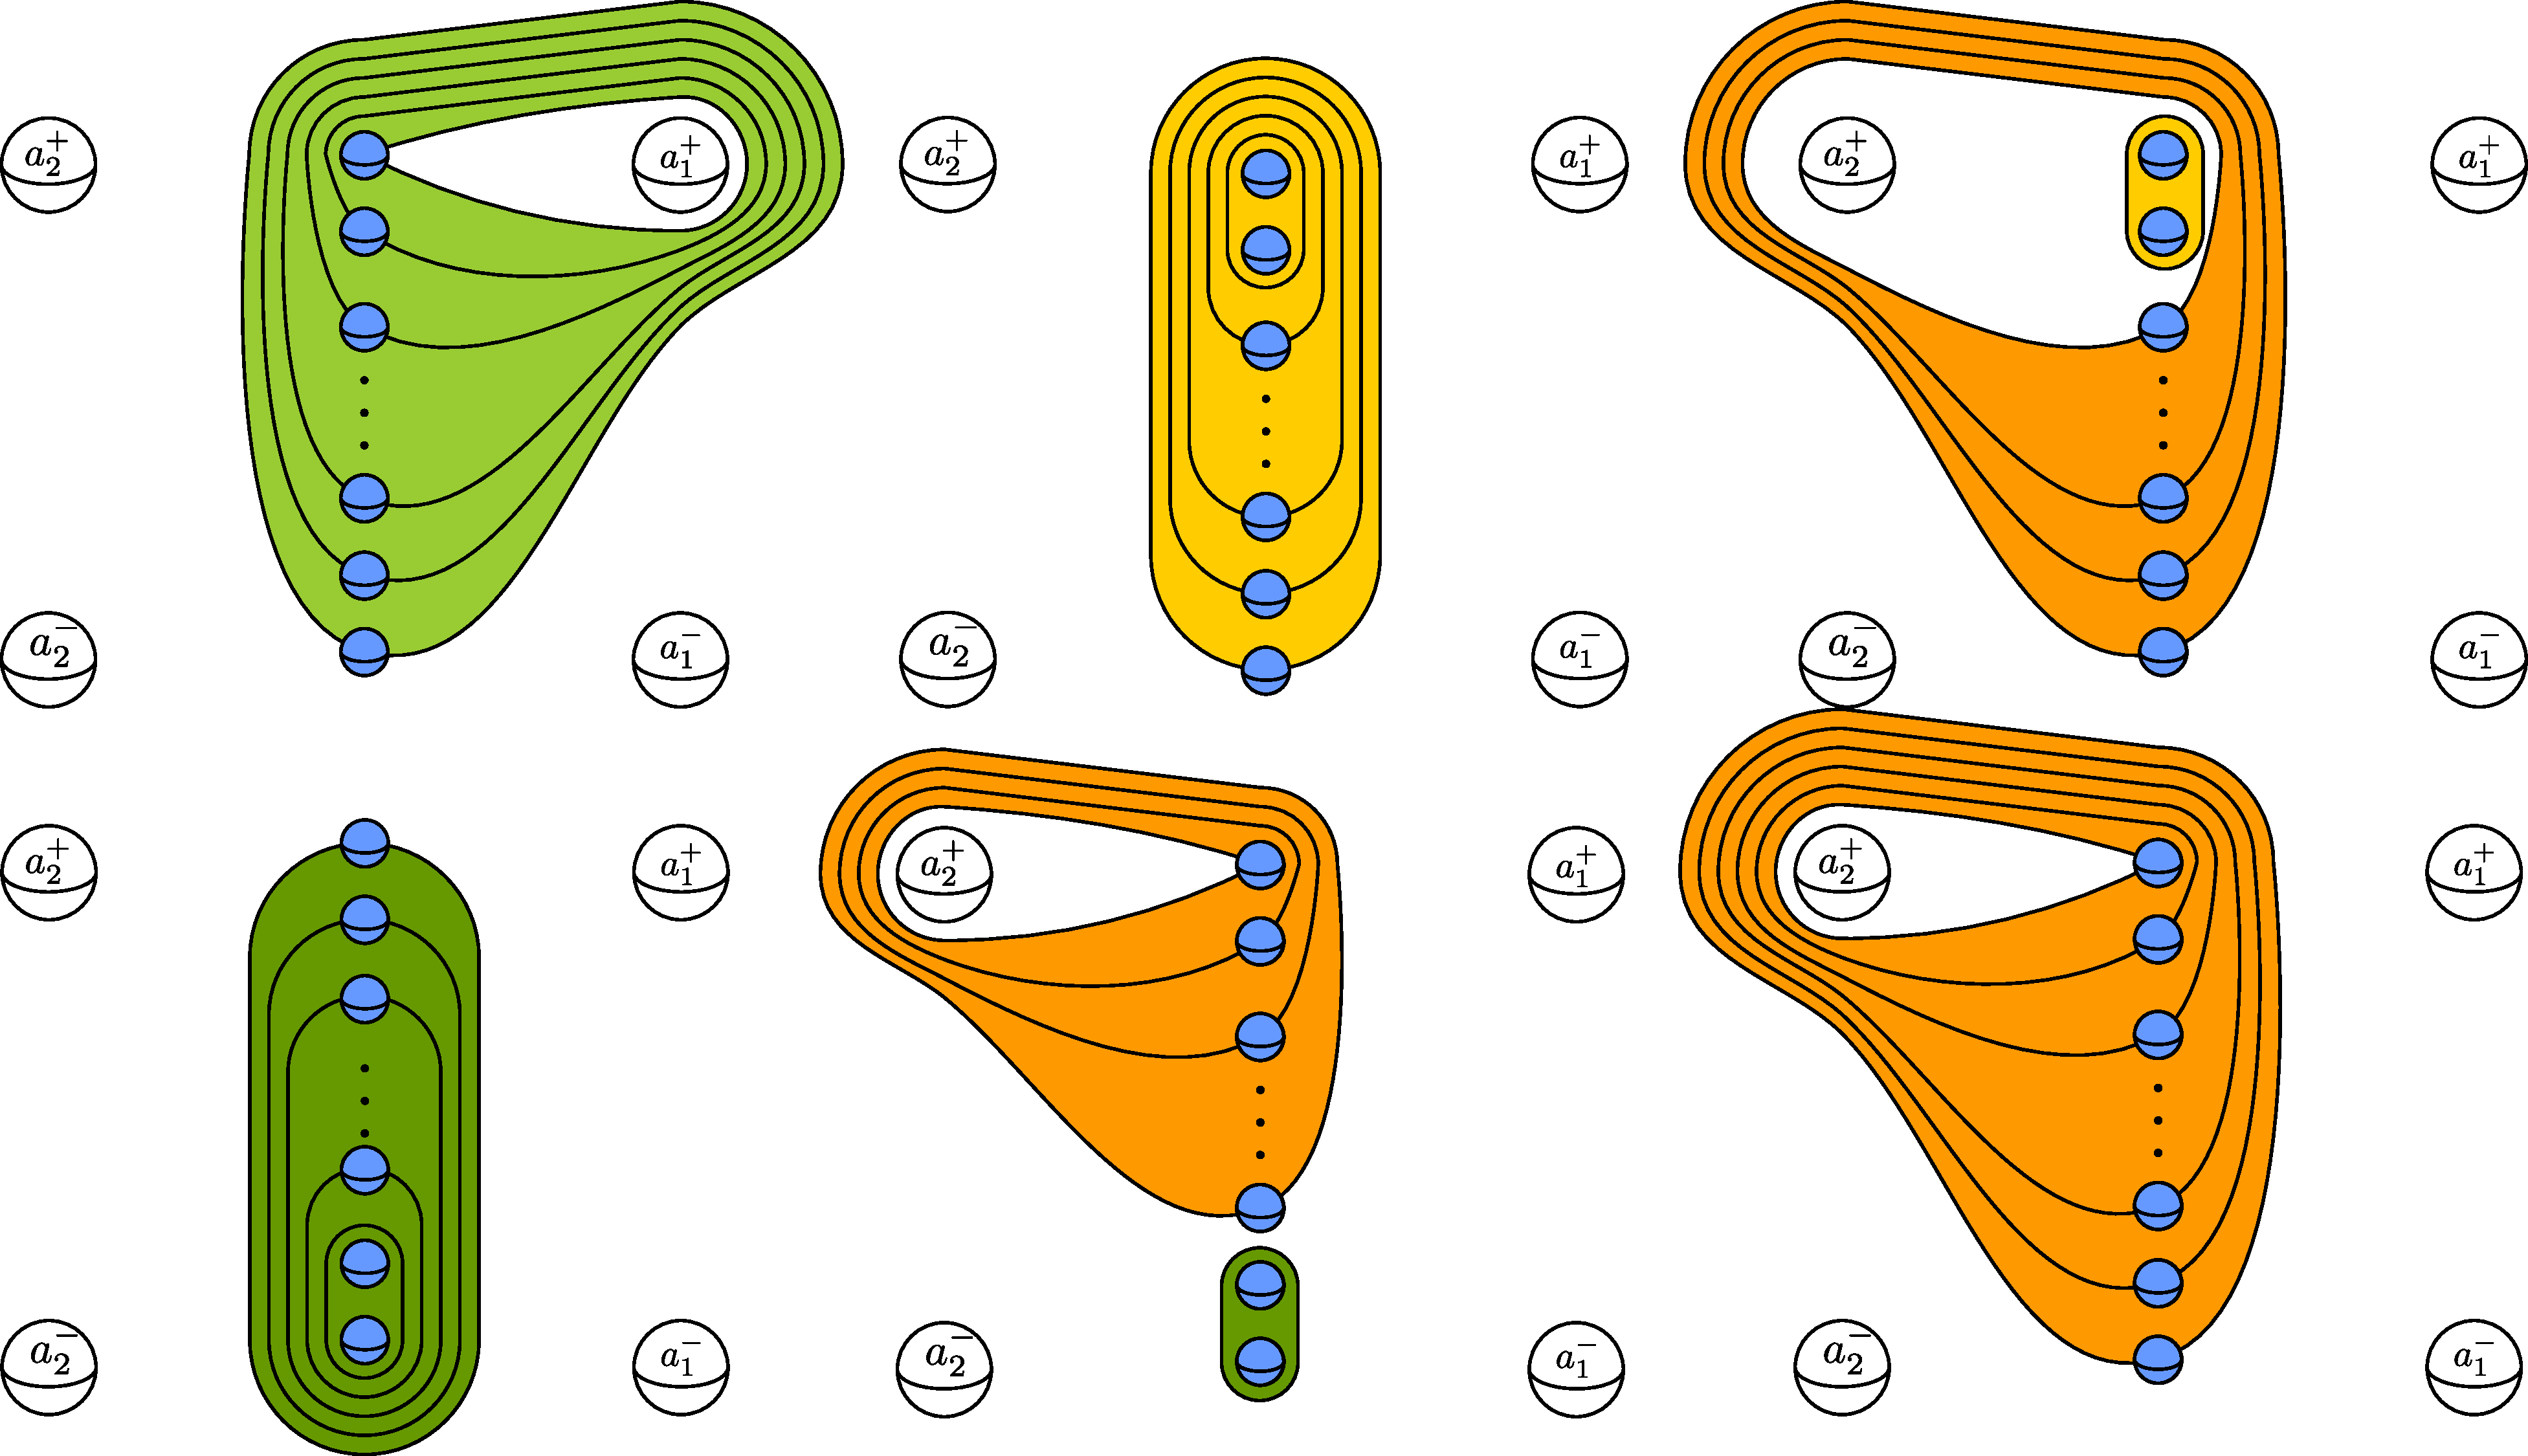
\includegraphics[width=\textwidth]{figures/ptspheretransposition2.pdf}
      \caption{A $\sigma$-nest forces a coloring on $\sigma^b_1\sigma$ nest for transposition $\sigma^a_1$.}
      \label{fig:ptspheretransposition2}
    \end{figure}

    \item $b$-transposition.
    Consider first the transposition $\sigma^b_1$.
    Figure \ref{fig:ptspheretransposition} shows a sequence of forcing colorings $\sigma^b_1$
    The argument for $\sigma^b_i$ is similar.

    \begin{figure}[h!]
      \centering
      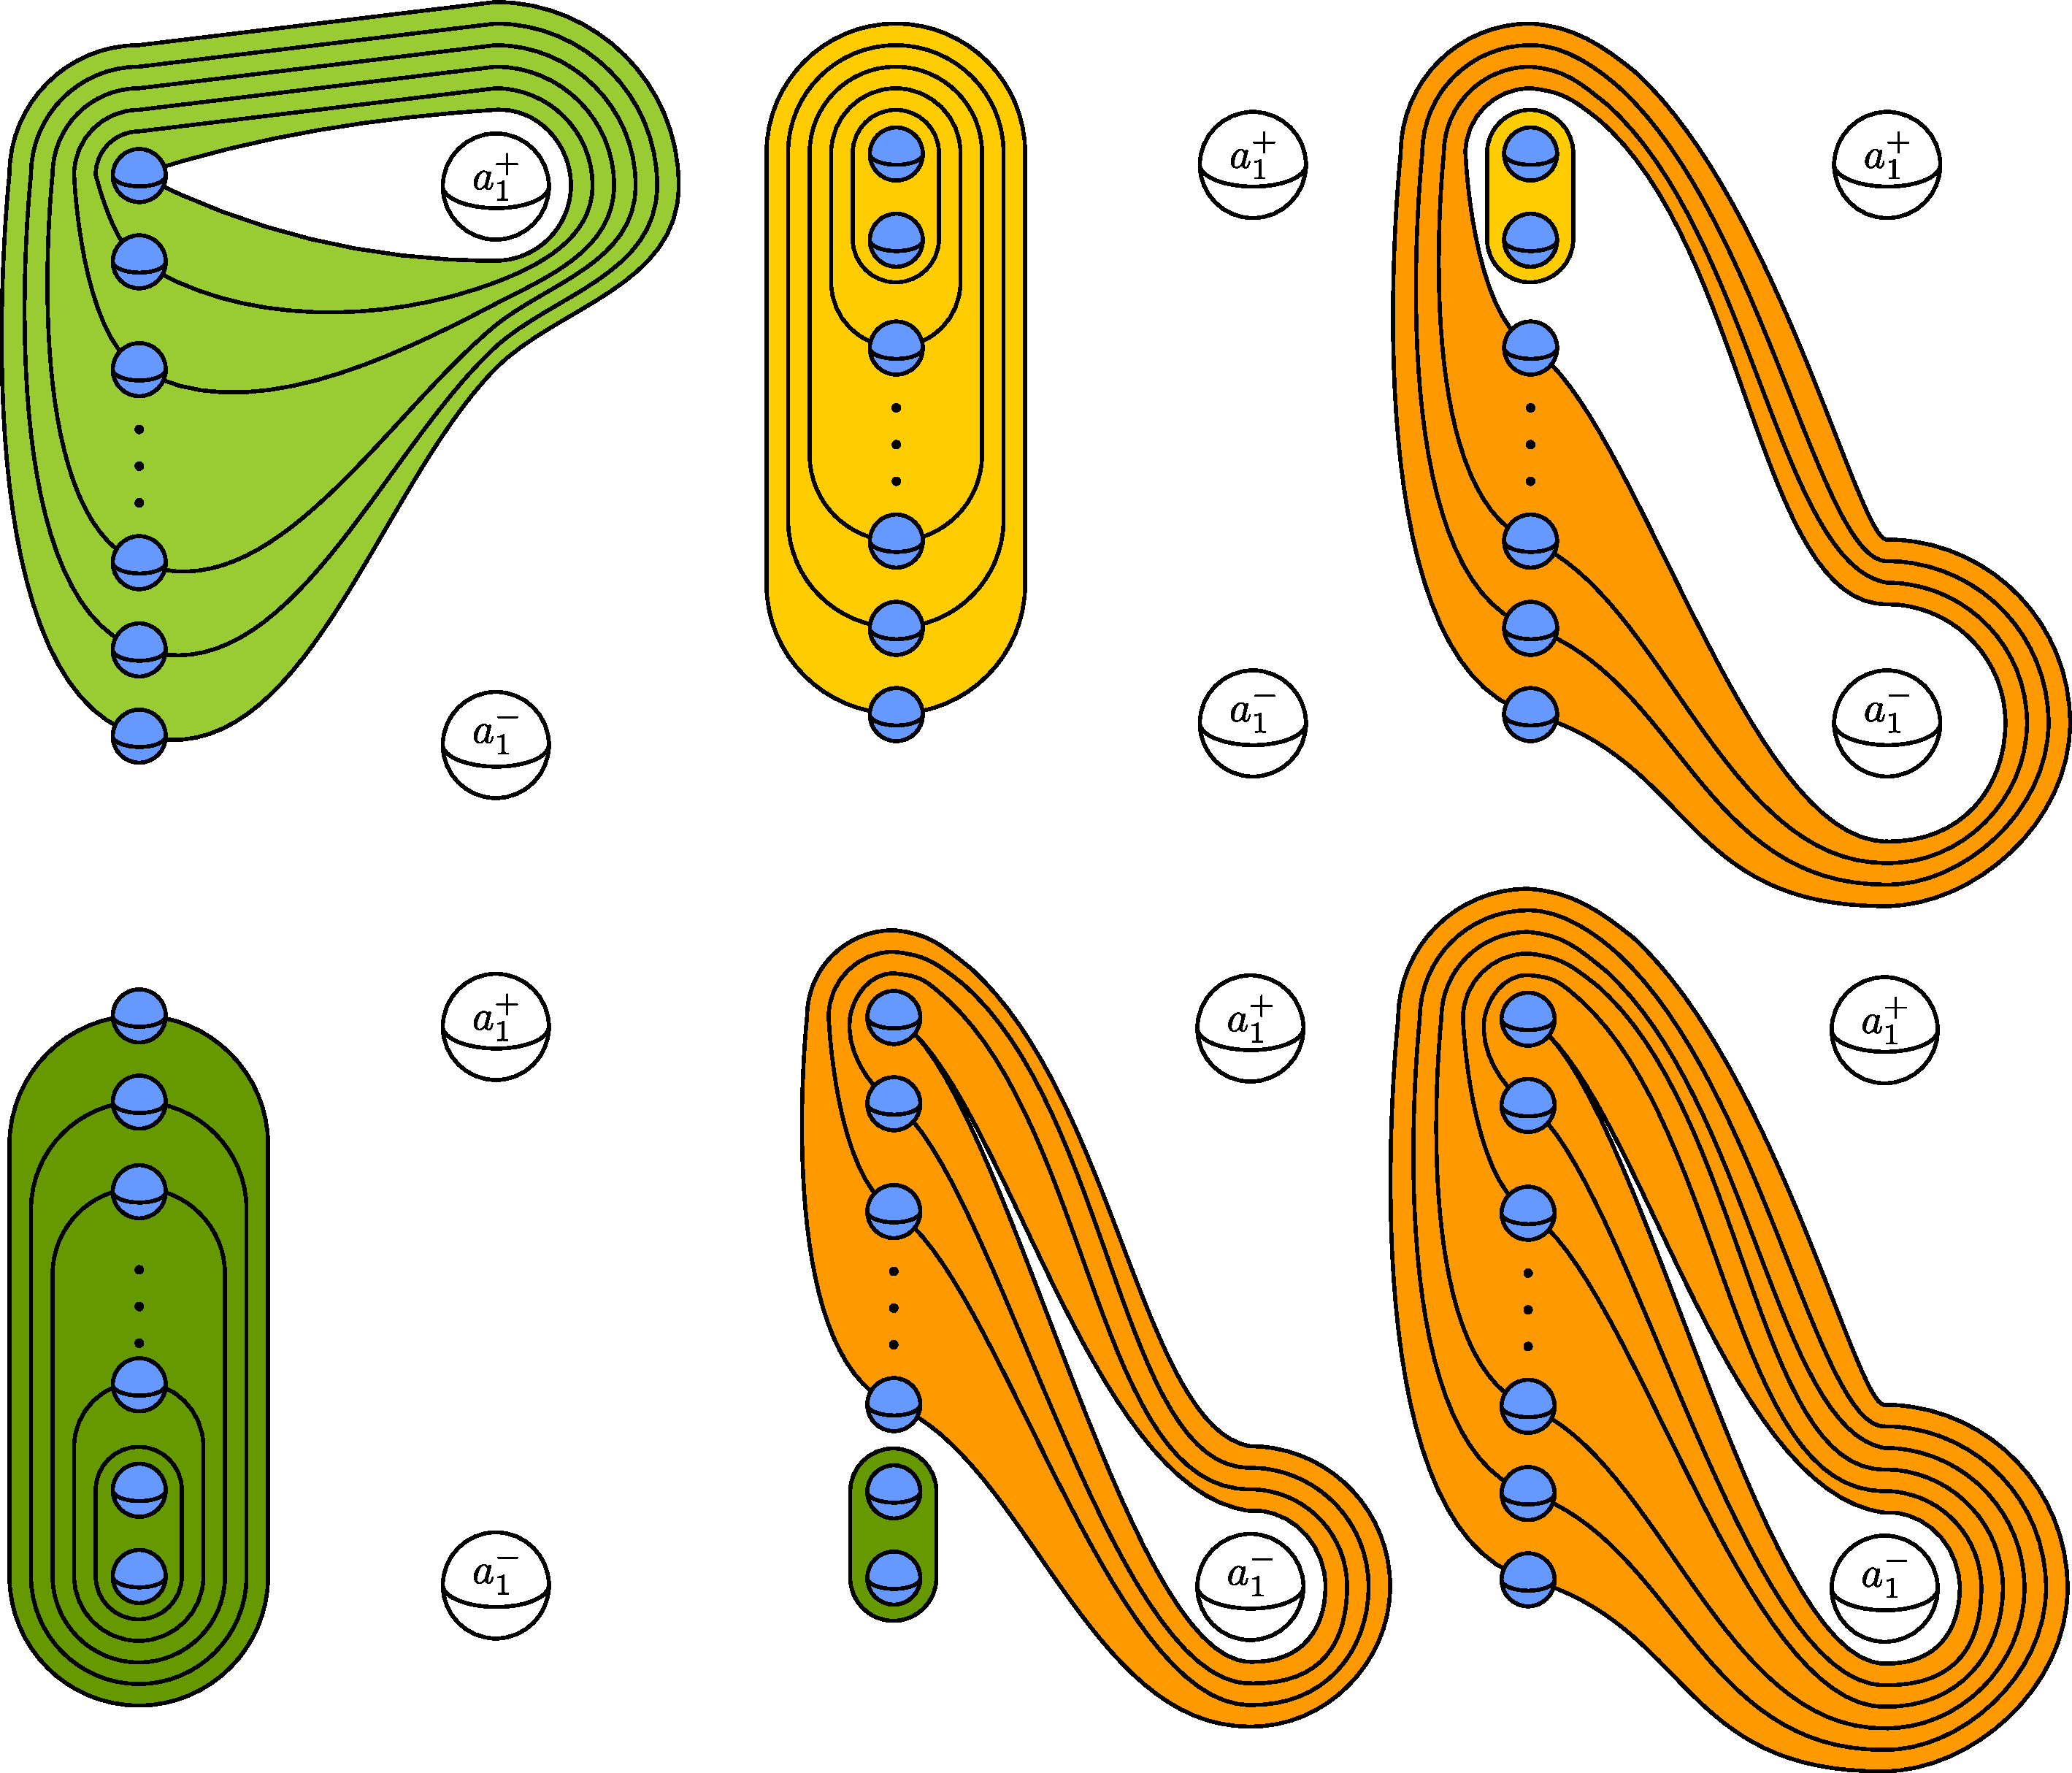
\includegraphics[width=\textwidth]{figures/ptspheretransposition.pdf}
      \caption{A $\sigma$-nest forces a coloring on $\sigma^b_1\sigma$ nest for transposition $\sigma^b_1$.}
      \label{fig:ptspheretransposition}
    \end{figure}

    \item Inversion. If $n>1$ then the inversion $\iota_2$ leaves $V$ fixed.

    If $n=1$ then Figure \ref{fig:ptsphereinversion} shows a sequence of coloring forcing.
    The first sequence forces a coloring on $\{v_{1,2},  \iota_1 v_3, \ldots, \iota_1 v_p\}$.
    The first sequence forces a coloring on $\{\iota_1 v_1, \ldots \iota_1 v_{p-2}, v_{p-1,p}\}$.
    So $V$ forces a coloring $\iota_1 \cdot V$.

    \begin{figure}[h!]
      \centering
      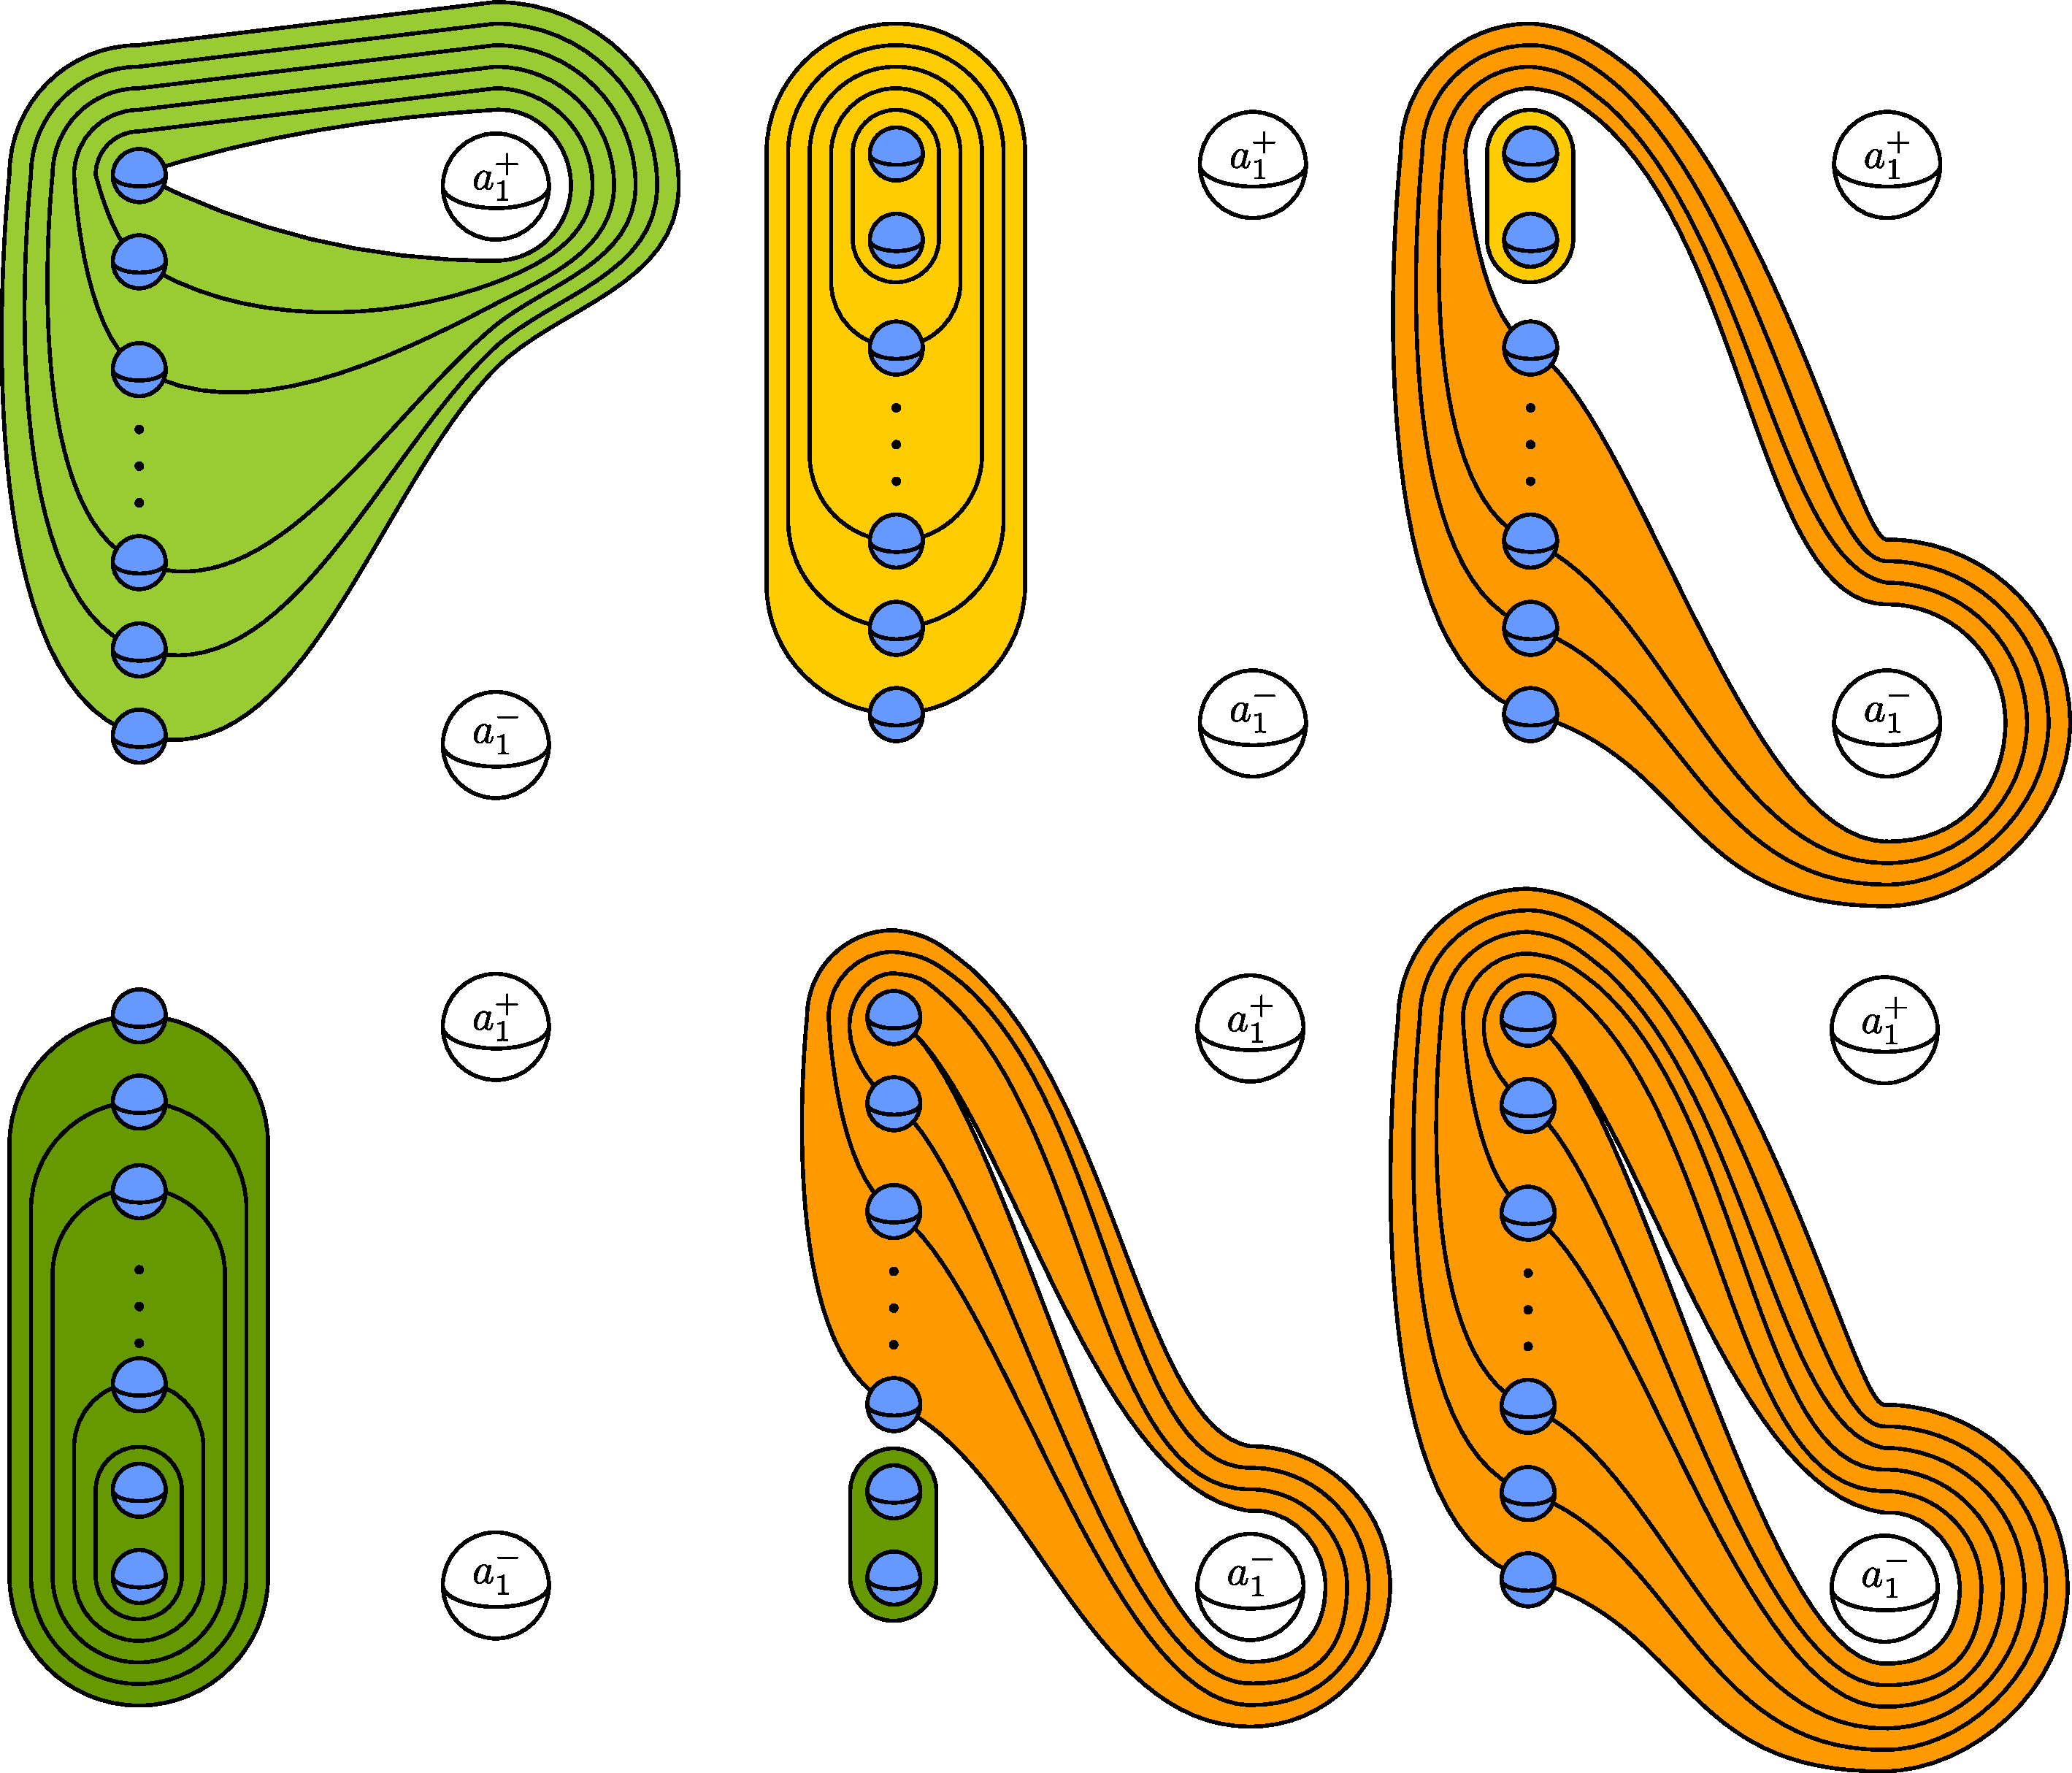
\includegraphics[width=\textwidth]{figures/ptsphereinversion.pdf}
      \caption{Two sequences together show the nest $V$ forces a coloring on $\iota_1V$.}
      \label{fig:ptsphereinversion}
    \end{figure}

    \item Conjugation. Figure \ref{fig:ptsphereconj} shows a sequences of forced colorings between
    $k$-colored simplices intersecting in $k-1$-colored simplices.
    from $V$ to $\tau_{12} \cdot V$.
    The case for $\tau^{-1}_{12}$ is similar.

    \begin{figure}[h!]
      \centering
      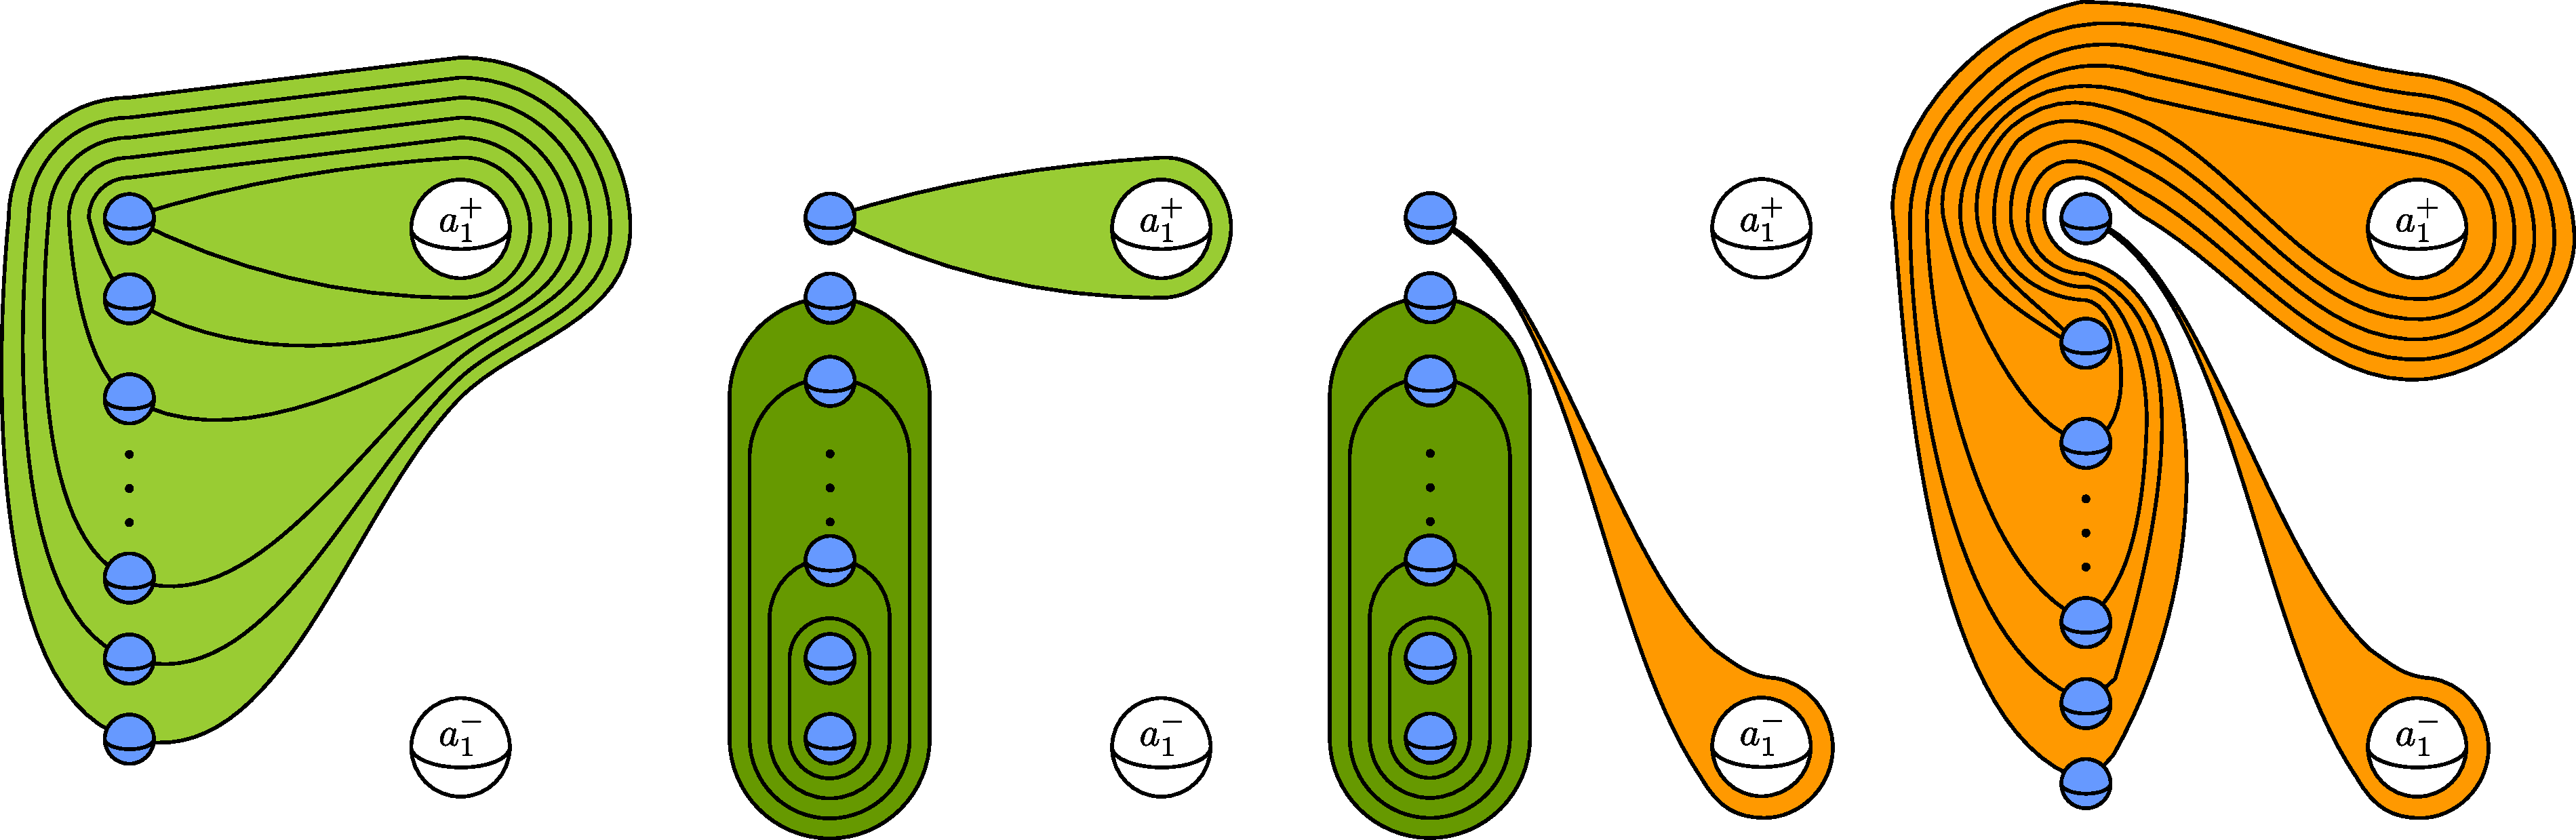
\includegraphics[width=\textwidth]{figures/ptsphereconj.pdf}
      \caption{The nest $V$ forces a coloring on $\tau_{12}V$.}
      \label{fig:ptsphereconj}
    \end{figure}
  \end{enumerate}
  From this we have that $V$ forces a coloring on its orbit $\oout_{n,p} \cdot V$.

  Finally we argue that $\oout_{n,p} \cdot V$ forces a coloring on $\mathcal S_{n,p}$.
  Let $V_k \subset \mathcal{PS}_{n,p}^{(0)}$ be the set of all
  unpointed separating spheres bounding $M_0,3$ and
  pointed separating spheres bounding $M_{0,j}$ for $j\leq k$.
  If $x \in V_3$, then we may find a collection of $k-2$ pointed nonseparating spheres that are
  disjoint from each other and from $x$.
  Then since $\oout_{n,p} \cdot V$ contains all pointed nonseparating spheres the coloring is determined on $x$.
  So $\oout_{n,p} \cdot V$ forces a coloring on $V_3$.
  Inductively we have that $V_k \cup \oout_{n,p} \cdot V$ forces a coloring on $V_{k+1} \cup \oout_{n,p} \cdot V$.
  So $V$ forces a coloring on $V_{p-1} \cup \oout_{n,p} \cdot V$.
  Then if $x$ is any pointed separating sphere,
  there are $p-1$ pointed curves or separating spheres bounding an $M_{0,3}$ that are mutually disjoint and disjoint from
   $x$.
  So $V_{p-1} \cup \oout_{n,p} \cdot V$ forces a coloring on $x$.
  Since $x$ was an arbitrary separating sphere, $V_{p-1} \cup \oout_{n,p} \cdot V$.
  The result then follow from Lemma \ref{putmancolor}.
\end{proof}

\begin{lemma}
  Sphere complex automorphisms induce automorphisms of the based sphere complex.

  There is a natural $\oout_{n,p}$-equivariant map
  $\aaut \mathcal S_{n,p} \to \aaut \mathcal{PS}_{n,p}$.
  \label{lemma:outbasedspheres}
\end{lemma}

\begin{proof}
  Let $\phi \in \aaut \mathcal S_{n,p}$ by an automorphism of the sphere complex.

  According to Lemma \ref{lemma:outspheretype} the automorphism $\phi$
  preserves the class of separating spheres bounding $M_{0,3}$.
  Suppose that $x$ is a pointed sphere of $M_{n,p}$.
  Then a regular $R$ neighborhood of $x$ is an $M_{0,3}$
  with a puncture and bounded by two spheres $x',x''$ of $M_{n,p}$.
  Observe that two spheres of $\mathcal S_{n,p}$ cobound an $M_{0,3}$
  with a puncture if and only if they are in a maximal simplex $\Delta$
  such that the corresponding vertex in the region adjacency graph $\mathcal G_\Delta$
  is degree 2.
  By Lemma \ref{lemma:outadjgraph} the adjacency graph $\mathcal G_{\phi(\Delta)}$
  is isomorphic to $\mathcal G_\Delta$,
  and $\phi(x')$ and $\phi(x'')$ bound a regular neighborhood of a punctured sphere $\hat \phi(x)$,
  and the map $x \mapsto \hat \phi(x)$ gives an isomorphism of $\mathcal {PS}_{n,p}$.
  Further $\phi \mapsto \hat \phi$ is an injection since every sphere of $M_{n,p}$
  is a boundary component for a regular neighborhood of some pointed sphere of $M_{n,p}$.
  Hence if $\hat \phi$ is the identity, so must $\phi$ be.
\end{proof}

\begin{lemma}
  Sphere complex automorphisms permute the fibers of the puncture forgetful map.
  Let $\phi \in \aaut \mathcal S_{n,p}$ and $x \in \mathcal S_{n,p}$.
  Then
  $$
  \phi \left ( \rho^{-1}_q\rho_q(x) \right )
  =\rho^{-1}_{q'}\rho_{q'}( \phi(x))
  $$
  for some $q' \in P$.
  \label{lemma:outfibers}
\end{lemma}

\begin{proof}
  Observe that an edge of $\mathcal S_{n,p}$
  in $\rho^{-1}_q\rho_q(x)$ specifies a punctured sphere of $\mathcal {PS}_{n,p}$
  colored by $q$.
  If $x,x' \in \rho^{-1}_q\rho_q(x)$ then we have a path
  $x=x_0, \ldots, x_n=y$ with $x_{i-1},x_{i}$  cobounding an $M_{0,3}$ that is the
  regular neighbodhood of punctured sphere $y_i$.
  Then by Lemma \ref{lemma:outbasedspheres} $\phi$ induces an automorphism $\hat \phi \in \mathcal{PS}_{n,p}$ such that $\phi(x_{i-1}),\phi(x_{i})$
  cobound a neighborhood of $\hat \phi(y_i)$.
  By Lemma \ref{lemma:outpaint} $\mathcal{PS}_{n,p}$ is uniquely colored by the punctures, so
  since $y_i$ are all colored by $q$ and $\hat \phi$ must permute the colors we have that
  $\hat \phi(y_i)$ are all punctured spheres based at the same point $q'$ and give the edges for the path
  $\phi(x_0), \ldots, \phi(x_n)$ in $\rho^{-1}_{q'}\rho_{q'}(x)$.
\end{proof}


\begin{proof}[Proof of Theorem \ref{thm:outpunc}]
Suppose that the natural map
$$
\begin{tikzcd}
\oout_{n,p-1} \arrow{r}{\gamma}& \aaut \mathcal S_{n,p-1}
\end{tikzcd}
$$
is an isomorphism.
Then according to Lemma
\ref{lemma:exactspheres} the following diagram commutes
$$
\begin{tikzcd}
1 \arrow[r]&
\pi_1(M_{n,p-1},q) \arrow[r] \arrow[d]&
\oout_{n,p}^{(q)}  \arrow{r}{f_q} \arrow{d}{\beta}&
\oout_{n,p-1} \arrow[r] \arrow[d]&
1 \\
1 \arrow[r]&
\pi_1(M_{n,p-1},q) \arrow{r}{\alpha}&
\aaut (\mathcal S_{n,p}, q)  \arrow{r}{\rho_{q}}&
\aaut \mathcal S_{n,p-1} \arrow{r}&
1 \\
\end{tikzcd}
$$
and has exact rows
since $\rho_q$ is a surjection as $\gamma f_q = \rho_q \beta$
is. By the Five Lemma we have $\beta$ is an isomorphism.
Let $\phi \in \aaut \mathcal S_{n,p}$.
By \ref{lemma:outfibers} $\phi$ permutes the fibers of the maps $\rho_q$,
so there is $\psi \in \oout_{n,p}$ such that
$\psi \phi$ preserves $\rho^{-1}_q \rho_q$.
But then  $\psi \phi \in \aaut \mathcal S_{n,p}^{(q)}$, and by the exact sequence
there is $\psi' \in \oout_{n,p}$ such that $\psi \phi=\psi'$.
But then $\phi = \psi^{-1} \psi'$ is also in $\oout_{n,p}$.
It follows that the natural map
$$
\begin{tikzcd}
\oout_{n,p} \arrow{r}{\gamma}& \aaut \mathcal S_{n,p}
\end{tikzcd}
$$
is an isomorphism.
\end{proof}
